% The \phantomsection command is needed to create a link to a place in the document that is not a
% figure, equation, table, section, subsection, chapter, etc.
%
% When do I need to invoke \phantomsection?
% https://tex.stackexchange.com/questions/44088/when-do-i-need-to-invoke-phantomsection
\phantomsection


% Multiple-language document - babel - selectlanguage vs begin/end{otherlanguage}
% https://tex.stackexchange.com/questions/36526/multiple-language-document-babel-selectlanguage-vs-begin-endotherlanguage
\begin{otherlanguage*}{brazil}

    \chapter[Experimentos]{Experimentos}


    \begin{flushright}
         
    \end{flushright}

    % \newpage

\section{Primeiros Experimentos}

Partindo desta pesquisa inicial, procurei desenvolver alguns experimentos musicais iniciais.  Por um lado, tinham as tecnologias de programação, que estavam surgindo naquele momento, mas também havia um repertório e teorias da música que se colocavam com meu ingresso no Doutorado. Esses primeiros estudos que eram projetos bastante simples, foram importantes como exercícios estéticos e para começar um aprendizado dessas novas tecnologias.


\subsection{Bandas Críticas}
Bandas Críticas pode ser considerada a primeira ``peça'' musical que escrevi. Até então, fazia apenas ``música''. Foi um primeiro exercício de escrita de uma partitura gráfica e o primeiro exercício de composição para uma equipe tocar. A peça foi composta a partir da proposta apresentada pelo Estúdio Fita Crepe \footnote{O Estúdio Fita Crepe foi um espaço dedicado à produção e performance de música experimental na cidade de São Paulo. \url{http://www.estudiofitacrepesp.com/}} de através do músico Ricardo Garcia ao NuSom, de um concerto de ``Música Silenciosa'', que seria uma ``música para acariciar os ouvidos'' que se embasaria em sutilezas de timbres e volumes.

A proposta foi de explorar metalinguisticamente o conceito de bandas críticas da audição, como apontamos em uma proposta de apresentação para o Simpósio Brasileiro de Computação Musical de 2015, que ocorreu em Campinas:


\begin{citacao}
A peça explora as frequências centrais e limítrofes das bandas críticas da audição, sobrepondo harmônicos e criando dissonâncias a partir de sons fora das escalas musicais tradicionais. Surge de um processo de composição metalinguístico, de investigar a própria percepção acústica, em um desejo de materialização de conceitos psicoacústicos em objetos sonoros. 
Surge de um processo de composição metalinguístico, de investigar a própria percepção acústica, em um desejo de materialização dos conceitos psicoacústicos em objetos sonoros. No caso, representa uma materialização do conceito de bandas críticas, buscando explorar sensações audíveis e artefatos emergentes da exploração desse conceito. A performance é programada para 3 músicos, cada um conectado a uma caixa de som diferente, para enfatizar as diferenças entre as frequências exploradas. \cite{ArianeStolfi2015}
\end{citacao}

Também foi uma experiência de composição abstrata, a partida da idéia de buscar uma saturação sensória formada a partir de frequências puras mas não necessariamente harmônicas, que fosse estimular todas as regiões da cóclea. A peça é estruturada em quatro partes, um primeiro movimento introdutório onde os músicos não performam e o processamento acontece de forma automatizada por um \emph{patch} de PD (Figura \ref{bandaspatch}), com todos os 44 osciladores ligando em um volume ascendente; um segundo momento, os músicos vão desligando os osciladores de acordo com uma ordem pré-estabelecidas, causando uma rarefação, até restarem apenas poucos osciladores ligados; na terceira parte os músicos improvisam a partir de harmônicos desses osciladores ligados; por fim, há um momento de ``destruição da onda'', onde os músicos passam a improvisar desenhando a onda, o que gera uma harmonia de ruídos, até a destruição completa dessas harmonias com a busca do silêncio.

\begin{figure}[htb]
    \caption{\label{bandaspartitura}Partitura gráfica para a peça Bandas Criticas. }
    \begin{center}
    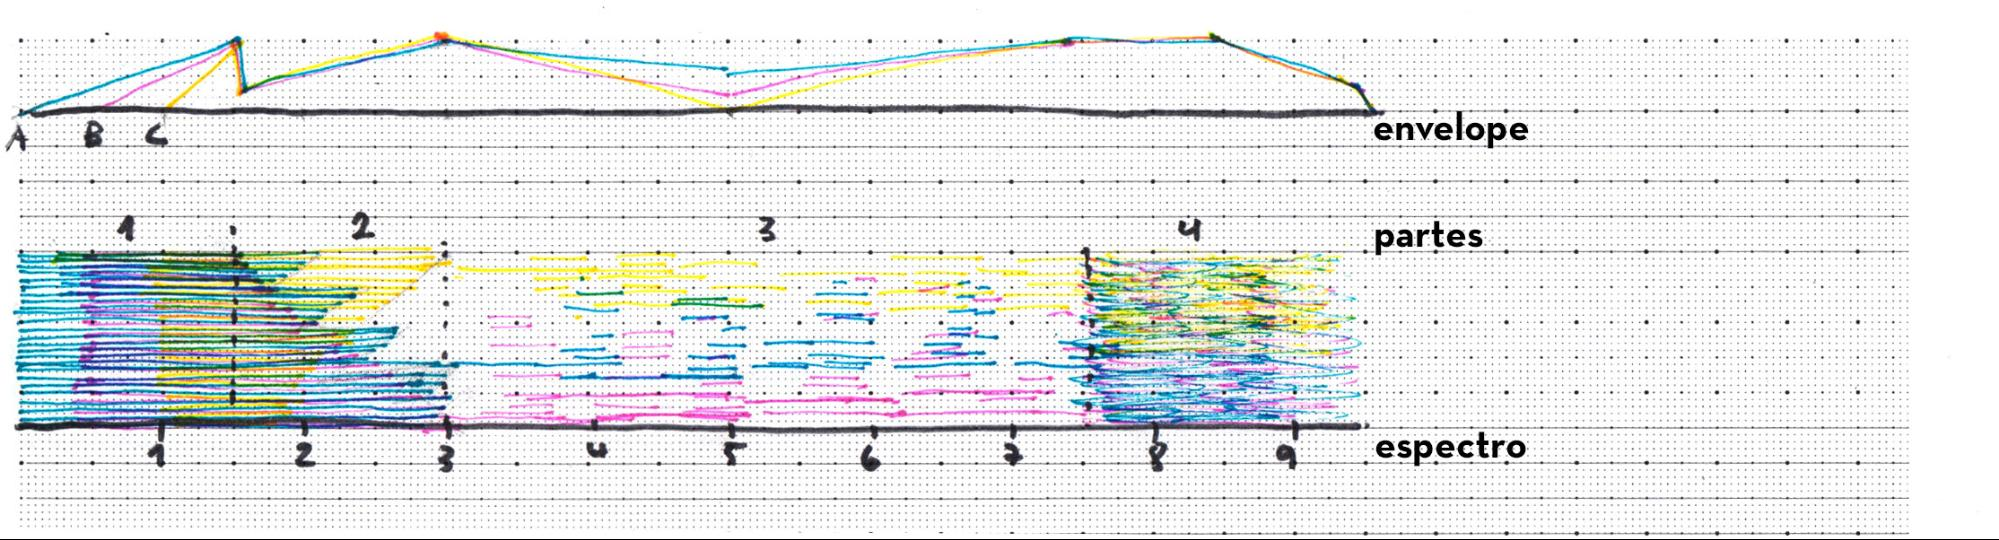
\includegraphics[width=1\linewidth]{pictures/cap3/bandascriticaspartitura}
    \end{center}
    \legend{Fonte: Screenshot da autora, Janeiro de 2016}
\end{figure}

Fizemos uma apresentação no Estúdio Fita Crepe, no evento ``Música? 11'', onde performaram junto comigo Davi Donato e Sérgio Abdalla, no dia 29 de agosto de 2015 e outra no Simpósio Brasileiro de Computação Musical no dia 24 de novembro em Campinas, com a participação de Davi Donato e Luzilei Aliel. Análise do registro das gravações mostraram que o espectrograma da peça ficou bem próximo ao desenho da partitura pensado originalmente, como podemos ver na imagem \ref{bandasciticasspec}. 

\begin{figure}[htb]
    \caption{\label{bandaspatch}Patch para a peça Bandas Criticas. }
    \begin{center}
    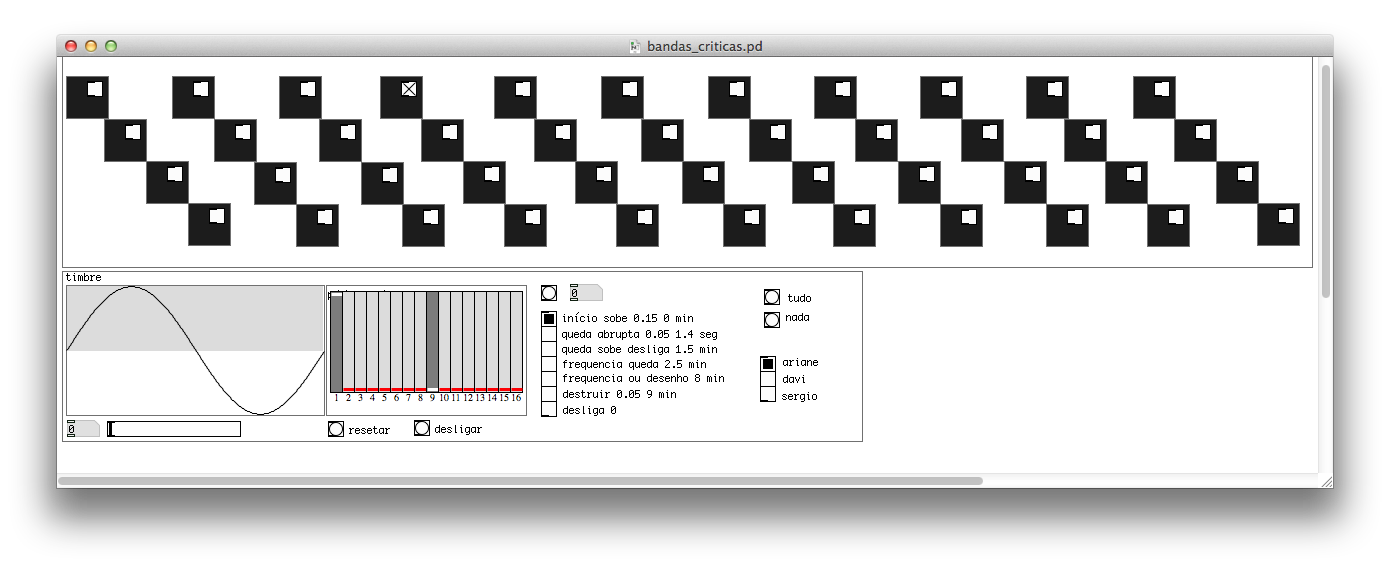
\includegraphics[width=1\linewidth]{pictures/cap3/bandascriticaspd}
    \end{center}
    \legend{Fonte: Screenshot da autora, Janeiro de 2016}
\end{figure}

\begin{figure}[htb]
    \caption{\label{bandasciticasspec}Espectrogramas gerados a partir das gravações da peça no Estúdio Fita Crepe (acima) e no SBCM (abaixo). }
    \begin{center}
    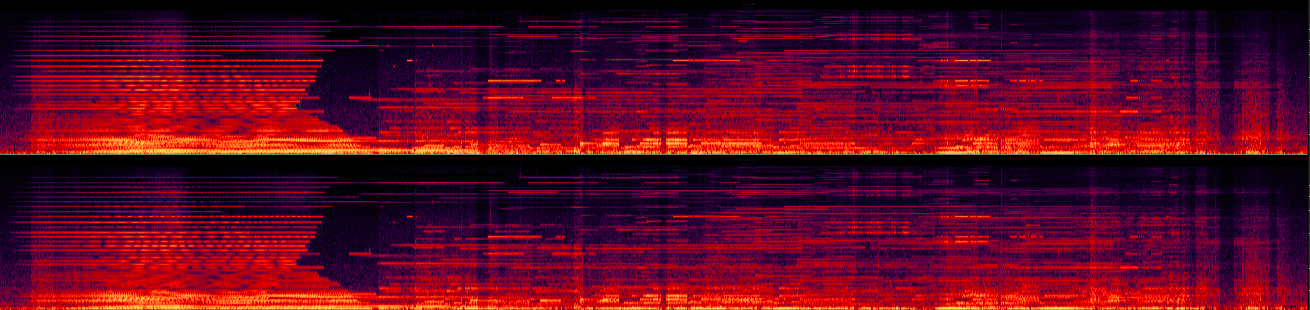
\includegraphics[width=1\linewidth]{pictures/cap3/bandascriticasspectro2}
    \end{center}
    \legend{Fonte: Screenshot da autora, Janeiro de 2016}
\end{figure}



\subsection{QWERTY}
\label{sec:QWERTY}
Qwerty foi o primeiro experimento em web áudio desenvolvido após entrar no programa de doutorado. Como a idéia inicial do projeto era buscar formas de explorar os inputs dos computadores pessoais, partimos da principal forma de input que é o teclado QWERTY, que tem a disposição ainda das tradicionais máquinas de escrever. A idéia era transformar o teclado em uma máquina sonora, que não é em si uma coisa nova. O site Patatap, por exemplo, que mencionamos no capítulo anterior, é uma plataforma que funciona dessa maneira. Outro exemplo é o ``Typedrummer'' de Kyle Stetz \footnote{Disponível em: \url{http://typedrummer.com/}} , onde o usuário digita um texto, e para cada letra há um sample, e o texto é tocado em loop.


Para essa máquina, me inspirei nas leituras de Haroldo de Campos do seu poema épico Galáxias \cite{Campos2004}, que tem como estrutura um bloco contínuo de frases sinestésicas, sem qualquer tipo de pontuação ou espaçamento. 

Naquele momento, estava envolvida também no projeto de digitalização das revistas de poesia concreta Código \ref{codigo}, da revista de vanguarda lançada em 1973 e editada por Erthos Albino de Souza e Antônio Risério, que contém obras e traduções de vários poetas concretos desta geração. A revista Código, é como aponta Augusto de Campos ``acolheu materiais de vanguarda que não encontrariam guarida nas publicações convencionais alternativas" \cite{Scandurra2016}. Para a versão online da revista, para o qual programei a interface, seguindo uma idéia de design de navegação paratática, ou seja, que permitisse a re-combinação e re-montagem dos poemas de acordo com a vontade do leitor. Por conta deste projeto, estava em contato constante com as obras dos poetas desta geração, então partimos a pesquisa desta inspiração.

Parti do poema Galáxias porque ele é sobretudo extremamente sonoro. O livro acompanha um CD com as leituras de Haroldo de alguns fragmentos do seu texto, e foi de onde partimos para a extração dos primeiros samples, buscando uma otimização do discurso, em uma relação com a própria estrutura do poema, que como apontou o poeta Augusto de Campos em conversa com a autora, poderia ter tido sua primeira edição publicada em folhas soltas para ser recombinado, ideia que foi abandonada posteriormente.

\begin{figure}[htb]
    \caption{\label{codigo}Interface do site da digitalização da revista Código. }
    \begin{center}
    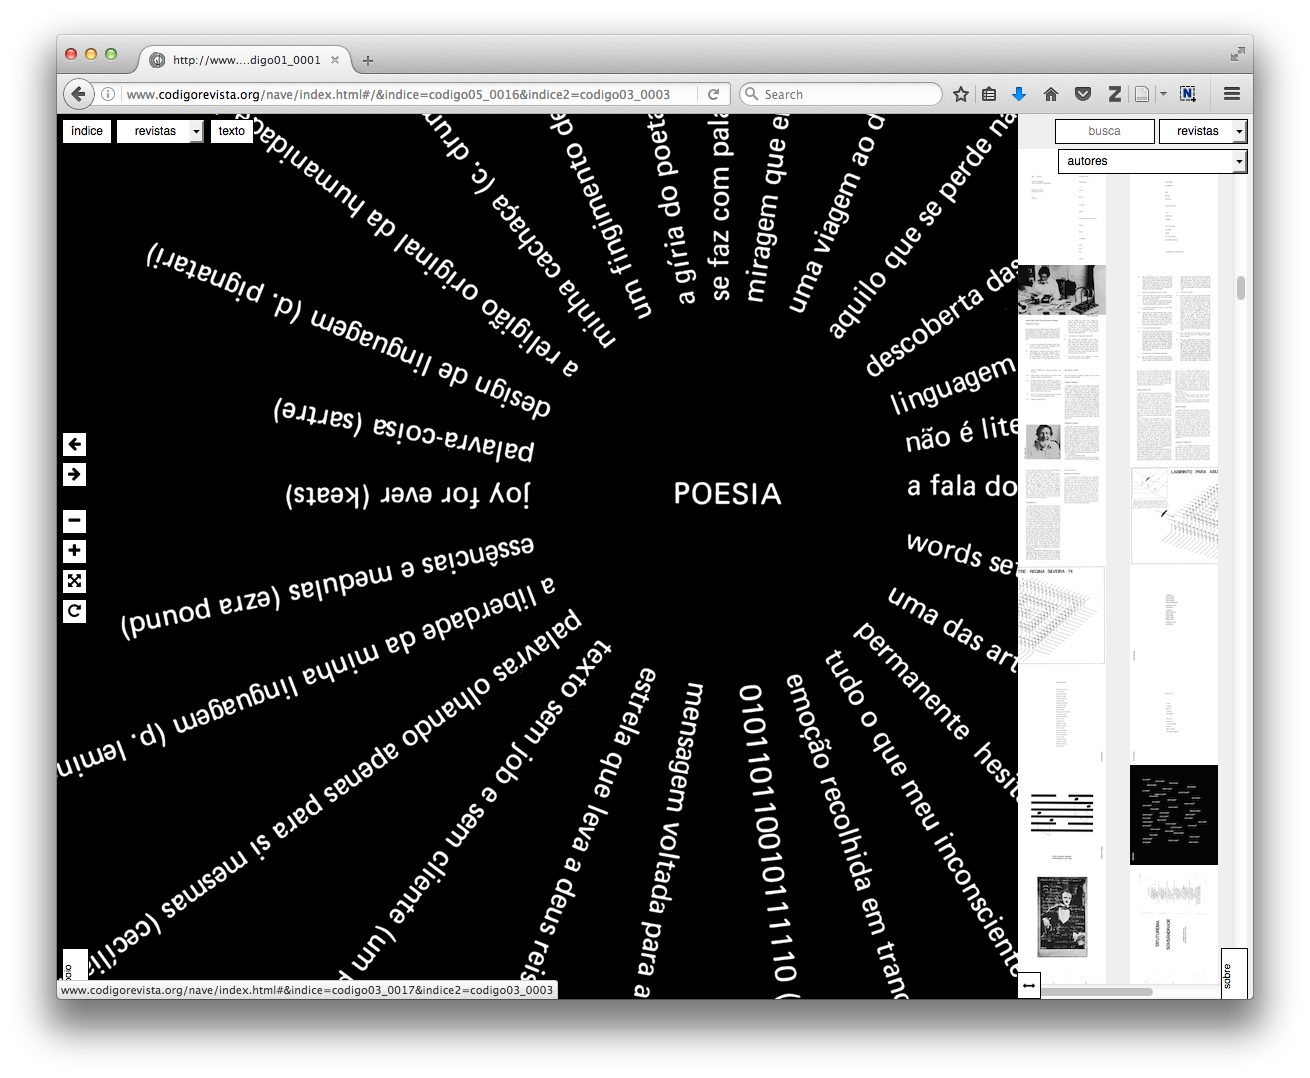
\includegraphics[width=1\linewidth]{pictures/codigo5.png}
    \end{center}
    \legend{Fonte: Screenshot da autora, Janeiro de 2016}
\end{figure}

Partimos de um processo de escuta buscado encontrar os sons correspondentes a cada letra em forma de token nas leituras do poeta e fizemos um mapa onde cada letra digitada do teclado corresponde a um fonema relacionado, criando um sampler de 26 botões, que são disparados ao digitar.

A interface desenvolvida foi a mais enxuta possível (figura \ref{qwerty}), pensando em um minimalismo radical que se relaciona com a estética da poesia concreta, e também em uma idéia de brutalismo digital que defendemos nesta pesquisa.

\begin{figure}[htb]
    \caption{\label{qwerty}Interface do experimento QWERTY, com fragmento de texto do Galáxias digitado. }
    \begin{center}
    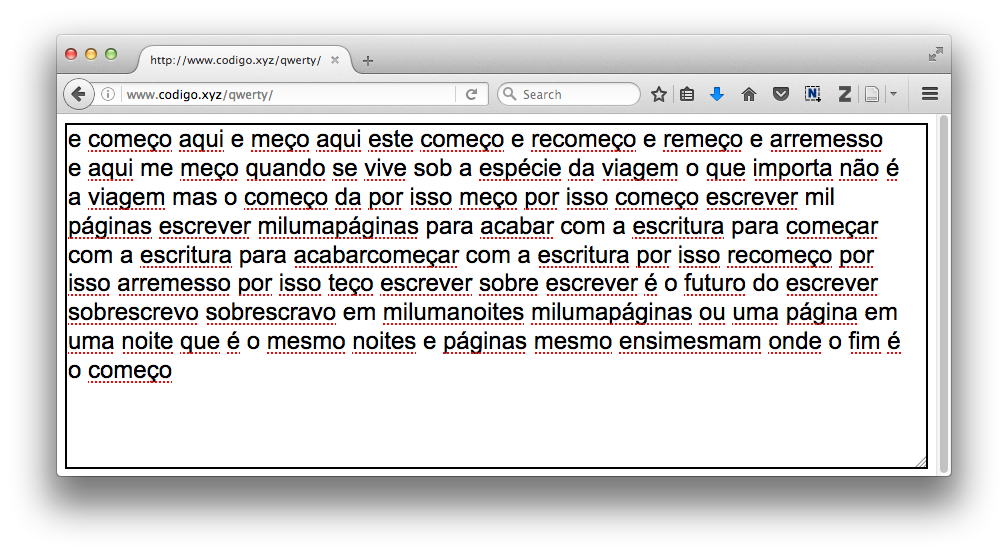
\includegraphics[width=1\linewidth]{pictures/qwerty.png}
    \end{center}
    \legend{Fonte: Screenshot da autora, Janeiro de 2016}
\end{figure}





\subsection{Protesta Fora Temer}
Durante o mês de outubro de 2016, surgiu uma discussão na lista de emails da rede sonora sobre a possibilidade de se posicionar contra o impeachment da presidenta Dilma Rousseff, após uma breve discussão, verificou-se a dificuldade de elaborar um texto que fosse consenso entre as pessoas da rede, devido à ausência de um debate qualificado sobre o assunto e a divergência de opiniões políticas. 
Surgiu então a proposta de organizar um protesto sonoro, e foi lançado um pedido na lista, pela compositora Valéria Bonafé, para quem quisesse participar, que enviasse algum sample em mp3: 
\begin{citacao}
Conversei com algumas membras aqui da Sonora e propus que a gente organizasse um protesto-sonoro-fora-temer. Nossa ideia é montar um protesto sonoro colaborativo e interativo a partir de samples de áudio. O convite está aberto a todo mundo aqui da lista! Quem quiser participar basta enviar um (ou mais!) sample(s) de áudio. As indicações técnicas são apenas duas: que seja curto (questão de alguns segundos) e que esteja em MP3. A ideia é fazer algo leve (no sentido técnico) para não sobrecarregar o sistema de interação que vamos usar para articular esse banco de samples. Como relação ao conteúdo, a única coisa que combinamos é que o mot é “fora temer”. Mas também não precisa ser literal! Não é que precisa gravar apenas falando “fora temer”. Pode ser! Mas pode ser também algo em torno disso. Enfim, temos um tema. Mas cada um pode pensar algo a partir disso. O uso da criatividade, da imaginação, da exploração, da experimentação, da espontaneidade e tudo mais está em aberto! Assim como a “forma”. Pode ser uma gravação nua e crua, pode ser processada, por ser um recorte de algo etc. Enfim, a única diretriz de conteúdo é “fora temer” e a única diretriz técnica é “um sample curto e leve”.
\end{citacao}
Várias pessoas da lista mandaram contribuições e a partir do material enviado, e propus que fizéssemos, ao invés de uma faixa estática, um protesto sonoro interativo. Selecionei 25 samples de áudio e criei uma página html onde o movimento do mouse vai soltando aleatoriamente os samples cada vez que passa por cima de uma das palavras do site. O resultado pode ser uma massa de vozes – a maioria femininas – ou um coro protestante, dependendo da velocidade que o internauta percorre a página (figura \ref{protesta}). O site está disponível no endereço \url{http://www.sonora.me/protesta/foratemer/}. 

\begin{figure}[htb]
    \caption{\label{protesta}Protesta Sonora. }
    \begin{center}
    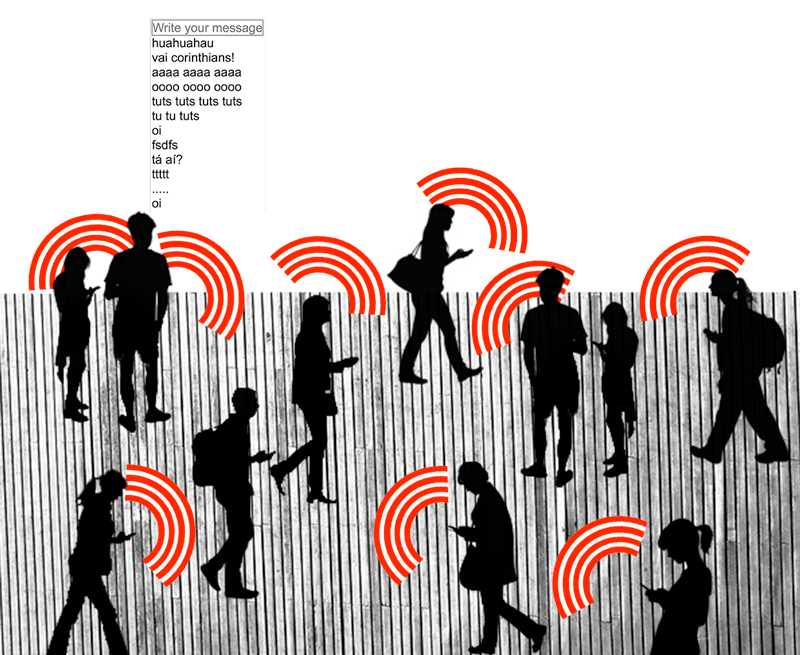
\includegraphics[width=1\linewidth]{pictures/banda_aberta_mob_crowd.png}
    \end{center}
    \legend{Fonte: Screenshot da autora dia 5 de janeiro de 2016}
\end{figure}



\section{Banda Aberta}
\begin{figure}[htb]
    \caption{\label{bandaabertamob}Banda aberta, imagem conceito para a proposta de intervenção pública}
    \begin{center}
    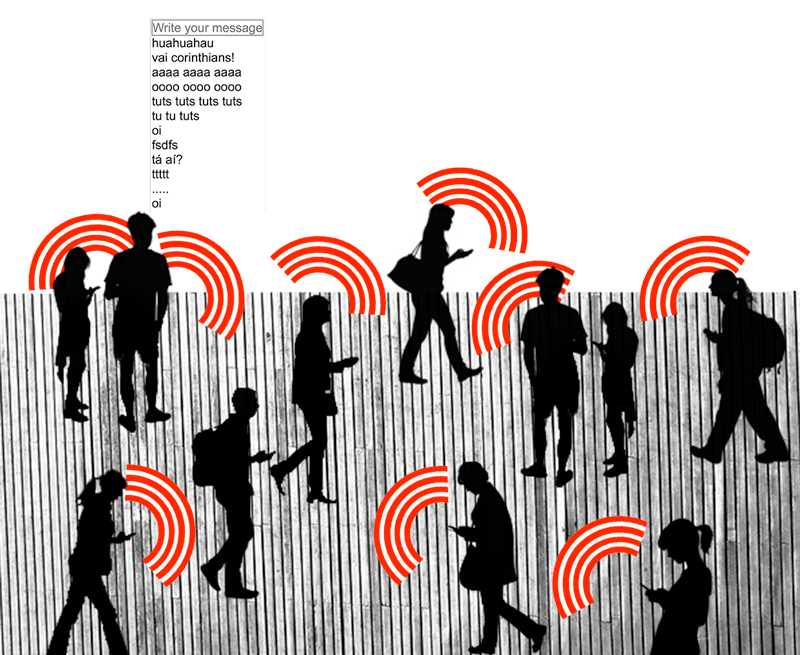
\includegraphics[width=1\linewidth]{pictures/banda_aberta_mob_crowd.png}
    \end{center}
    \legend{Fonte: desenho da autora}
\end{figure}

\subsection{Introdução}
O projeto Banda Aberta começou a ser desenvolvido como parte da proposta do NuSom para o Festival Bigorna na Praça, organizado pelo Estúdio Fita Crepe na praça José Molina. A ideia inicial era conectar os dispositivos pessoais das pessoas pela internet, de modo a potencializar os amplificadores individuais dos celulares e pensar em uma proposta de performance participativa que envolvesse a audiência. Foi o primeiro projeto realizado em parceria com outro programador, o engenheiro de computação Fábio Goródscy, que estava realizando mestrado na Computação musical no IME e o primeiro grande projeto desenvolvido no âmbito desta pesquisa. A parceria com um cientista da computação permitiu que desenvolvêssemos uma estrutura mais complexa do que a dos primeiros experimentos, que ainda eram baseados principalmente em HTML5, e partir para a exploração de recursos mais complexos da Web Audio API \cite{Adenot2015}.

O principal objetivo desta performance era o dar voz ao coletivo, liberdade de fala, criando possibilidades de comunicação musical sem significado. Visamos permitir que pessoas em um espaço público venham a interagir em um contexto musical, fazendo um espetáculo produzido por elas mesmas, sem necessidade de nenhum conhecimento musical, utilizando seus próprios celulares, via wifi através de um sistema \emph{open-source} de chat sonoro. A figura abaixo apresenta uma representação da performance em um ambiente aberto. 

Performance com participação da audiência mediada por tecnologia é um tópico emergente no campo da tecnologia musical \cite{wu2017open} e na esfera da arte contemporânea. Em contraste com performances tradicionais, onde há uma divisão estrita entre audiência e performer, as performances participativas tendem a diluir os limites entre a audiência e o performer \cite{kattwinkel2003audience}. 

Na tradição artística brasileira, esse assunto tem sido explorado desde os anos 60, principalmente no trabalho artístico de neoconcretos como Hélio Oiticica e Lygia Clark. Os parangolés de Oiticica, desenvolvidos a partir de um trabalho do artista com a comunidade da mangueira no final dos anos 60 eram peças vestíveis, cujo sentido se dava na dança e na manipulação das formas pela comunidade, assim como os Bichos, de Lygia Clark, que são esculturas articuladas que podem ser manipuladas e re-compostas pelo público. \cite{Braga2008}

Atualmente, o desenvolvimento da tecnologia trouxe novos recursos para facilitar e encorajar processos participativos em performances e instalações como: dispositivos computacionais portáteis como Arduino\footnote{Plataforma eletrôncia em código aberto Arduino: \url{https://www.arduino.cc/}} ou Bela{Plataforma para processamento de áudio de baixa latência Bela: \url{http://bela.io/}}; smartphones; sensores de dimensão reduzida e novas linguagens versáteis de alto nível como Python e JavaScript, que também ajudaram a criar as bases para o campo de pesquisa da computação ubíqua. Diversos projetos utilizam tecnologias deste tipo para o emprego criativo da participação da audiência em performances ao vivo, como os projetos massMobile \cite{Weitzner2012}, Mood Conductor \cite{Fazekas:2014}, Open Symphony \cite{wu2017open}, Crowd in Cloud \cite{Lee2016} e TweetDreams \cite{Dahl2011}. Em condições ideais, os participante são capazes de interagir durante as performances interferindo na narrativa de modo sensível. 

O projeto de ambientes colaborativos para produção musical pode ser desafiador, no sentido de que a audiência não necessariamente compartilha de domínio de técnicas e processos musicais. O projeto Banda Aberta é uma tentativa de explorar esse tema, usando a música como ponto de partida, pela função social que ela tem de comunhão e comunicação \cite{Koelsch:2014}. A idéia era de propor uma obra ``aberta'', como defendida por Umberto Eco \cite{Eco1991}, que, de acordo com Robey \cite{Eco1991}, requer do público um grau muito maior de envolvimento pessoal e colaboração do que qualquer obra de arte tradicional do passado. Segundo Eco, em uma obra aberta, ``é decisão do artista de deixar com que parte da organização de seus constituintes seja relegada ao público ou ao acaso, dando a elas assim não uma ordenação definitiva, mas uma multiplicidade de ordens possíveis" \cite{Eco1991}.

Com o projeto Banda Aberta, nós queríamos criar um sistema que pudesse ser facilmente utilizado como um instrumento musical pelos participantes, independente de qualquer conhecimento musical a priori. Existem vários tipos de interface para participação musical que partem de gestos de toque, simulando um processo de interação similar ao dos instrumentos tradicionais, como por exemplo a performance ``88 Fingers'' de Norbert Schnell e Benjamin Matuszewki \cite{Schnell2017}, onde cada participante pode controlar através do celular uma das teclas de um piano MIDI, ou ``Hyperconnected Action Painting", de Anna Xambó e Gerard Roma \cite{Xambo2017}, onde a audiência usa gestos com o celular para disparar sons pré definidos. Apesar de ambas serem divertidas como experiência participativa, o resultado sonoro nesses dois casos, na minha impressão pessoal, foi de uma massa de sons desordenada e fora de ritmo. Acredito que isso aconteceu em parte pela falta de prática em processos musicais coletivos por parte da audiência, que não necessariamente domina o gestual musical. Pensando nessa questão, queríamos propor uma ferramenta que pudesse ser acessada por qualquer usuário, independente de qualquer formação ou treinamento em práticas musicais, e para isso, procuramos partir de tecnologias que as pessoas já usam com mais desenvoltura.

\subsection{Descrição do Projeto}
Como já apontava McLuhan\cite{mcluhan1968comunicaccoes}, o alfabeto fonético é uma tecnologia fundamental para o desenvolvimento da cultura ocidental. Ele é fácil de se aprender e ajustável a várias linguagens, sendo assim, a base de toda cultura literata. Neste trabalho, nós fazemos uso do alfabeto como tecnologia para produzir música experimental. Texto e mensagens instantâneas se tornaram a principal forma de comunicação nos celulares hoje em dia, seja em comunicações síncronas ou assíncronas \cite{Madell:2007}, e por isso, decidimos experimentar com  o texto através de mensagens como forma de interação musical nesta primeira proposta. Muitos tipos de interfaces para produção musical usam o texto como forma de \emph{input}, como nos processos de \emph{live coding} \cite{Collins2003}, em processos participativos que usam feedback verbal da audiência \cite{noauthor_transglasphone_nodate}, em composições algorítmicas geradas por dados textuais ou sistemas que usam o teclado como controlador musical \cite{Fiebrink2007}. Neste projeto, nós procuramos criar um sistema que funcionasse para a produção musical de uma maneira análoga à relação entre o alfabeto e a linguagem oral.

A comunicação \emph{online} por texto se aproxima muito da comunicação oral, pela facilidade de escrita, e pela velocidade quase instantânea,\cite[33]{Levinson2001} Como aponta McLuhan, o conteúdo de um meio sempre agrega um meio anterior. O discurso, que é o meio mais antigo, está contido em quase todos meios subsequentes, como o livro, o telégrafo, o cinema e a televisão, e, é claro, a internet \cite[42]{Levinson2001}. 

McLuhan aponta que o espaço visual surge quando as consoantes foram criadas, ``como uma abstração sem significado", permitindo a análise das unidades silábicas em cada um de seus componentes. A consoante é para ele um não-som, algo que necessariamente ``soa junto". \cite[13-14]{mcluhan1968comunicaccoes} A base do discurso, segundo ele é o fonema, a unidade mínima do som, que seria a unidade mínima do som, na música, no entanto, Tenney  propõe em ``Meta-Hodos and Meta Hodos" o conceito de ``clang", que seria uma unidade \emph{gestalt} mínima reconhecível \cite[23]{Tenney1988}. 

Neste projeto, ao buscarmos o som das consoantes de um modo isolado, criamos uma desconstrução do discurso e procuramos reforçar esse caráter atomizante da linguagem escrita através de um duplo processo de conversão: discurso convertido em texto e posteriormente convertido em música.

A digitação é um processo muito mais simples para a maioria dos usuários de computadores e dispositivos digitais, em relação à operação de interfaces musicais, assim como a digitação na máquina de escrever era mais acessível para o homem comum do que o tocar de instrumentos analógicos. \cite[172]{Levinson2001}. Nossa ideia foi utilizar o \emph{input} de texto como forma de interação musical. 

Num projeto realizado previamente, o QWERTY, já tinha começado a explorar a digitação como forma de input, mapeando cada letra do teclado para um sample, que eram disparados de acordo com a digitação. Nós percebemos que isto exige do performer uma certa habilidade de controle do gesto, para que os sons saiam em um ritmo definido. Além disso, como as interfaces dos \emph{smartphones} não facilitam a digitação, queríamos pensar um sistema que não dependesse de agilidade para funcionar. Para encorajar a participação, nós projetamos um sistema que funcionava a partir de simples mensagens de texto.

No nosso projeto, utilizamos as frases como disparadores para uma sequência de samples, que são já compostos com durações fixas, num processo análogo ao de composição de frases musicais. Ao colocar um mecanismo de chat, as pessoas podem acessar o instrumento simultaneamente e participar de um diálogo sonoro. Conforme mais pessoas vão escrevendo simultaneamente, a camada de samples se torna mais densa e entrópica.

Diferente de processos de síntese vocal, nosso chat não concatena as sílabas, somente toca os sons pré-determinados em uma sequência, de modo que as palavras não são compreendidas como palavras, mas como frases musicais. Para adicionar um certo grau de controle à performance, utilizamos uma lógica da interface por linha de comando, através de certos comandos especiais que podem alterar a dinâmica da peça, ou alternar entre os conjuntos de samples compostos.

O projeto é construído a partir de dois dispositivos, o servidor de mensagens, que é programado em \emph{Ruby} e necessita de instalação em um servidor web, e a interface que faz o processamento das mensagens e é construída em HTML e \emph{JavaScript} e funciona a partir da Web Audio API. O sistema está disponível como código aberto\footnote{O código fonte está disponível em: \url{https://github.com/fabiogoro/bandaserver}}   

\begin{figure}[htb]
    \caption{\label{bandaabertaserver}Diagrama esquemático dos servidores do projeto Banda Aberta}
    \begin{center}
        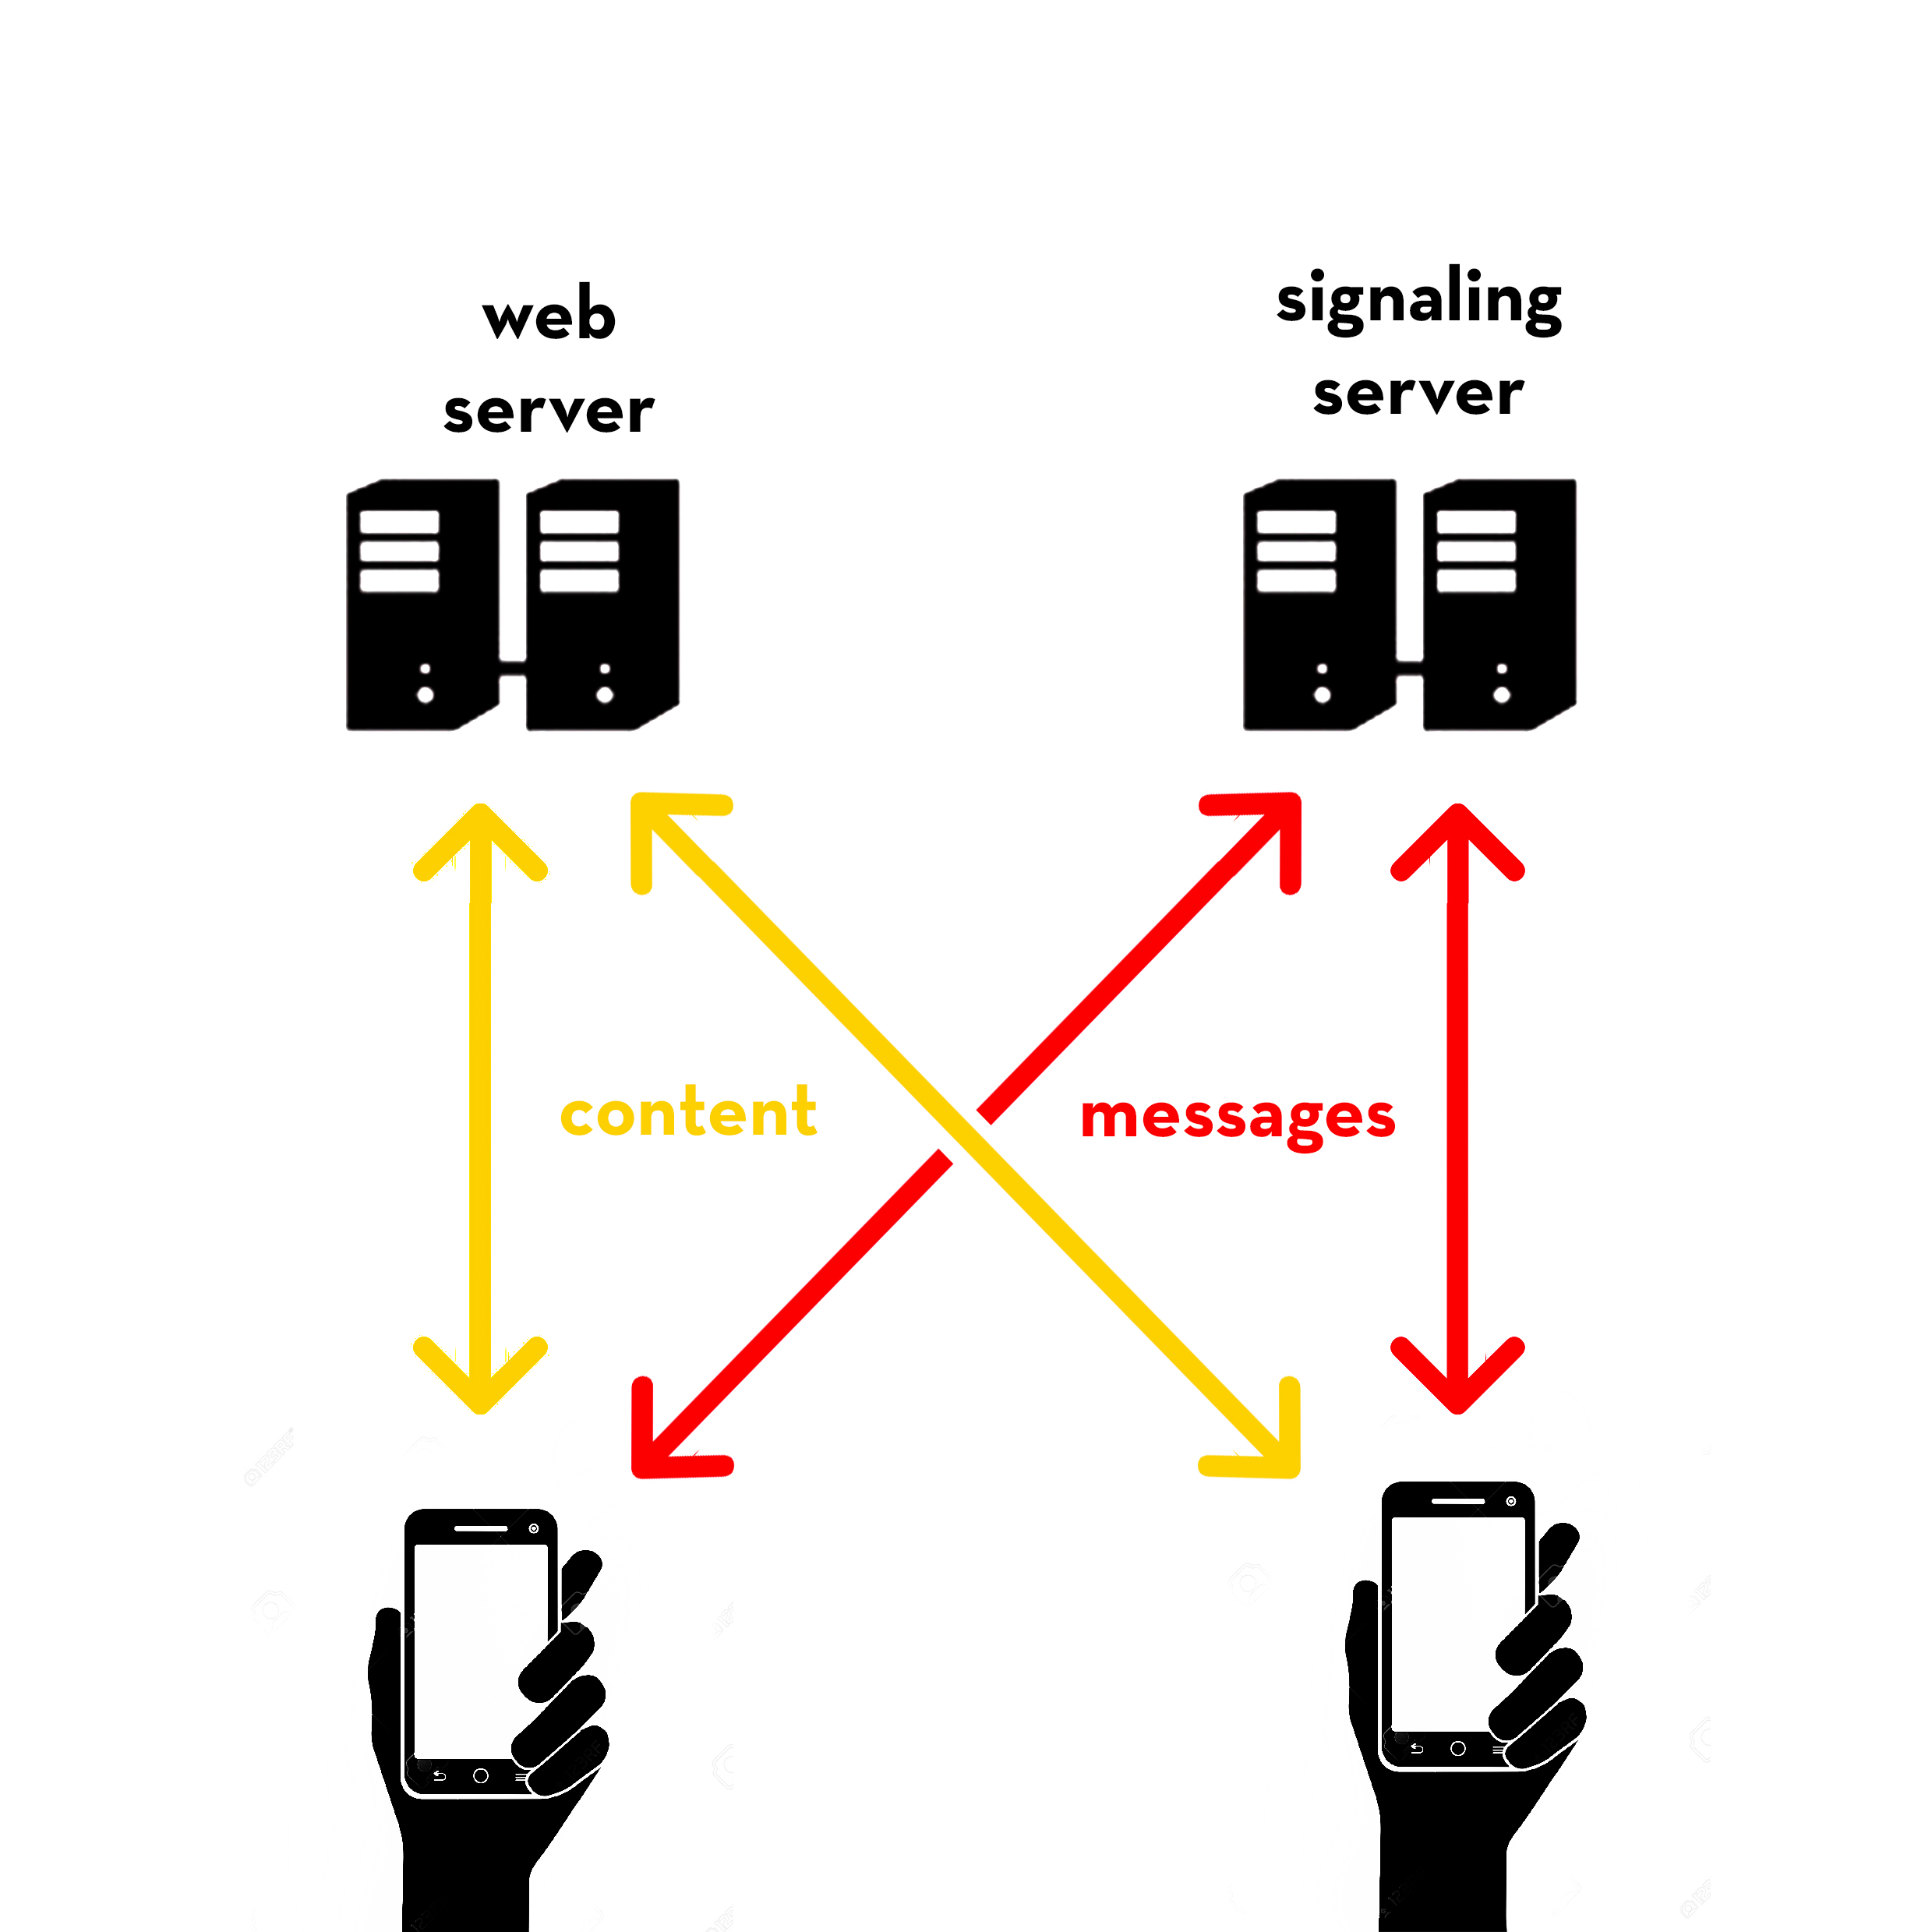
\includegraphics[width=0.5\linewidth]{pictures/server.jpg}
    \end{center}
    \legend{Fonte: desenho da autora}
\end{figure}

Na primeira versão, o processamento de áudio funciona somente por sampleamento. Os samples são numerados de acordo com a tabela ASCII e estabeleci um sample para caractere da tabela. O sistema converte as letras nos números equivalentes segundo a tabela, e toca o sample respectivo segundo a ordem estabelecida por cada frase que é enviada ao chat. Posteriormente, desenvolvemos também uma segunda versão baseada somente em síntese que também funciona da mesma forma, com um mapeamento um-para-um, de um som para cada letra.

\subsection{Desenvolvimento do Projeto}
Para o desenvolvimento do projeto Banda Aberta, adotamos ``Lean UX'' como metodologia de design. Lean UX é uma metodologia ágil de desenvolvimento de software que tem sido aplicada em muitos projetos de webdesign \cite{leanux}. Envolve a criação de um protótipo mínimo e viável a partir de um estágio muito inicial do projeto. Este protótipo devem então ser testado em condições reais de uso e melhorias são feitas de modo iterativo, baseando-se em observações e feedbacks recolhidos. O projeto foi desenvolvido como software de código aberto e está disponível no Github. \footnote{Os códigos-fonte do projeto estão disponíveis em: \url{https://github.com/fabiogoro/bandaserver}}. A arquitetura do sistema foi descrita com mais detalhes no artigo publicado na conferência Audio Mostly de 2017 ``Open Band: A Platform for Collective Sound Dialogues''~\cite{Stolfi2017}.

Nosso primeiro protótipo contava apenas com o conjunto inicial de samples nomeado de ``Galáxias'', e pudemos testá-lo menos de um mês após a proposta inicial em uma reunião do NuSom. Os samples utilizados nessa primeira versão eram os mesmos reunidos para o experimento QWERTY, descrito na seção \ref{sec:QWERTY}. A experiência foi registrada e fizemos uma análise dos comentários dos participantes\footnote{Registro da experiência pode ser visto em: \url{https://www.youtube.com/watch?v=Utc_4mT5b8s}}. Pudemos notar desde o princípio que a performance tinha um certo grau de ludicidade, pelas reações de riso e divertimento dos presentes. 


Neste primeiro teste em público, notamos que haviam alguns problemas com relação à compatibilidade de aparelhos, que foram posteriormente corrigidos. Recebemos também a opinião de alguns usuários que notaram que após alguns minutos a experiência sonora passava a ser um pouco entediante, com a repetição constante dos mesmos sons. Propusemos então a criação de outros bancos de sons, que seriam alternados durante a performance, e que um deles fosse criado colaborativamente por um grupo de estudantes da Universidade Anhembi Morumbi, orientados pelo professor Vítor Kisil,  que também apresentariam uma peça no Festival Bigorna. A partir daí, compusemos os demais pacotes de samples discutidos na seção \ref{sec:trad}

Nós queríamos assegurar a acessibilidade da audiência e garantir uma flexibilidade na montagem da performance, garantindo seu funcionamento mesmo em locais sem disponibilidade de acesso à Internet, o que era o caso do Festival Bigorna. Para isso, utilizamos um roteador Wifi para criar uma rede local aberta onde os usuários podiam ter acesso ao sistema em um servidor local (esta prática é frequentemente utilizada como estratégia para permitir a participação da audiência em sistemas de música móvel\cite{Lambert:2016}). Uma questão em performances participativas via celulares é que muitas vezes os usuários podem se distrair durante a se usar internet em dispositivos celulares para performances participativas e que usuários frequentemente podem se distrair por informações vindas de outros aplicativos como de trocas de mensagens ou redes sociais\cite{wu2017open}, e isto também é evitado pela rede local, que isola os usuários da internet, deixando os mais focados na performance e na experiência resultante. Durante as performances, os participantes acessaram o sistema através de um endereço IP que direcionava para uma máquina local com o servidor.

Nossa intenção era de que os participantes pudessem interagir com pouca ou nenhuma explicação anterior. No começo das era passada somente instruções de qual endereço acessar, onde havia a informação ``envie sua mensagem''. O endereço IP e o nome da rede eram informado em uma projeção na tela (na maioria das performances) para auxiliar os participantes a entrar mesmo depois do início da mesma. Um site com uma versão online é mantido no ar desde o lançamento do projeto e pode ser acessado no endereço: \url{banda.codigo.xyz}




\subsubsection{Tradução Inter Semiótica}
\label{sec:trad}

O uso do teclado do computador como \emph{input} para produzir sons em instrumentos musicais digitais pode ser relacionado muitas vezes com o teclado de piano. A maioria dos softwares do tipo DAW, como o ``Logic Audio" ou o ``Pro Tools" propõe uma interface de ``digitação musical" onde o teclado pode ser usado como um controlador MIDI precário (no sentido de que não possui sensibilidade à pressão) que relaciona teclas a notas musicais determinadas. Neste paradigma, a associação entre letras e sons é geralmente arbitrariamente determinada pela posição das teclas do teclado em comparação com a posição das teclas do piano, sem nenhuma relação semântica entre o som gerado e as próprias letras. Neste projeto, queríamos manter uma relação semântica entre as letras utilizadas nas mensagens e o resultado sonoro gerado. Para isso, buscamos algumas formas de tradução inter-semiótica entre os caracteres e os sons, que fosse além dessa analogia com as teclas de piano. A tradução semiótica é um procedimento utilizado para traduzir diferentes códigos, como aponta Plaza: 

\begin{citacao}
Na tradução intersemiótica como transcriação de formas o que se visa é penetrar pelas entranhas dos diferentes signos, buscando iluminar suas relações estruturais, pois são essas relações que mais interessam quando se trata de focalizar os procedimentos que regem a tradução. Traduzir criativamente é, sobretudo, inteligir estruturas que visam à transformação de formas. \cite[71]{JulioPlaza1969}
\end{citacao}

Aplicar um processo de tradução inter-semiótica de texto para som se relaciona com a idéia de áudio semântico \cite{Kostek:2010}, mas não no sentido tradicional, já que o objetivo aqui não foi o de dar sentido semântico aos sons, mas sim o de explorar quais poderiam ser os significados das letras quando essas fossem transformadas em sons. A abordagem foi de produzir os samples de acordo com o conceito de James Tenney \cite{Tenney1988} de Clang, ou ``gestalt aural", que é similar ao conceito de objeto celular de Pierre Schaeffer, que são objetos sonoros breves ou redundantes \cite{Chion1983}. A ideia foi pensar em átomos que pudessem ser recombinados livremente na medida em que as mensagens fossem escritas. Este procedimento aumenta as possibilidades paratáticas do sistema ao permitir re-combinações para além das possibilitadas pela linguagem escrita.


No sistema fonético, Schaeffer \cite{Schaeffer2007} aponta que as vogais em geral servem como sons de suporte e as consoantes como articulação. Segui esse princípio guia para o mapeamento das letras em sons, buscando cobrir uma grande variação de ``clangs", para deixar espaço para o acaso. Para a primeira versão do projeto, foram feitos 4 grupos de samples com sonoridades diferentes que podem ser mudados em tempo real por quem souber os comandos especiais: 

\begin{description}
 \item[Galáxias] A primeira estratégia foi de construir um alfabeto sonoro, usando processo de analogia com os sons do alfabeto fonético. Apesar de existirem muitos sistemas de síntese de discurso, a tentativa foi de isolar os sons, atomizando o discurso e consequentemente, o transformando em música através do encadeamento sucessivo de sons em uma estrutura rítmica. 
Em uma homenagem à poesia concreta, como definida por Augusto de Campos: ``tensão de palaras-coisas no espaço-tempo'' \cite[45]{campos_teoria_2014}, começamos a recortar os sons desse alfabeto a partir das leituras de Haroldo de Campos do Poema Galáxias \cite{Campos2004}, um poema épico longo que se situa entre a prosa e a poesia, com várias páginas de texto sem nenhuma divisão de parágrafos ou marcas de pontuação. Sua leitura calma e grave foi percebida como uma fonte rica para um conjunto consistente de sons, e dessas gravações conseguimos extrair um conjunto que cobriu todas as letras em caixa baixa. Para as letras maiúsculas, procurei buscar sons mais poderosos, parte dos quais retirei de uma demonstração de técnicas vocais estendidas gravada por Stênio Biazon e outros que gravei especialmente para isso usando minha própria voz.  

Para os caracteres, a relação direta entre os sons e os samples não é tão clara, uma vez que não são representações fonéticas, então optei por procurar outras relações possíveis bem como outras fontes de sons. Em alguns casos seguimos uma lógica de relação mais simbólica, como de caixa registradora para o signo \$ e em outros, associações mais icônicas, utilizando uma técnica de síntese subtrativa por corte visual de espectro. Este é o conjunto padrão de samples, e é usado como introdução para tornar as pessoas familiares com o sistema de associação. Exemplos deste pacote de sons podem ser ouvidos em: \url{http://spectro.codigo.xyz/spectrogramplayer/}

\begin{figure}[htb]
    \caption{\label{samplesgalaxias}Espectrogramas do Conjunto de Samples Galáxias}
    \begin{center}
        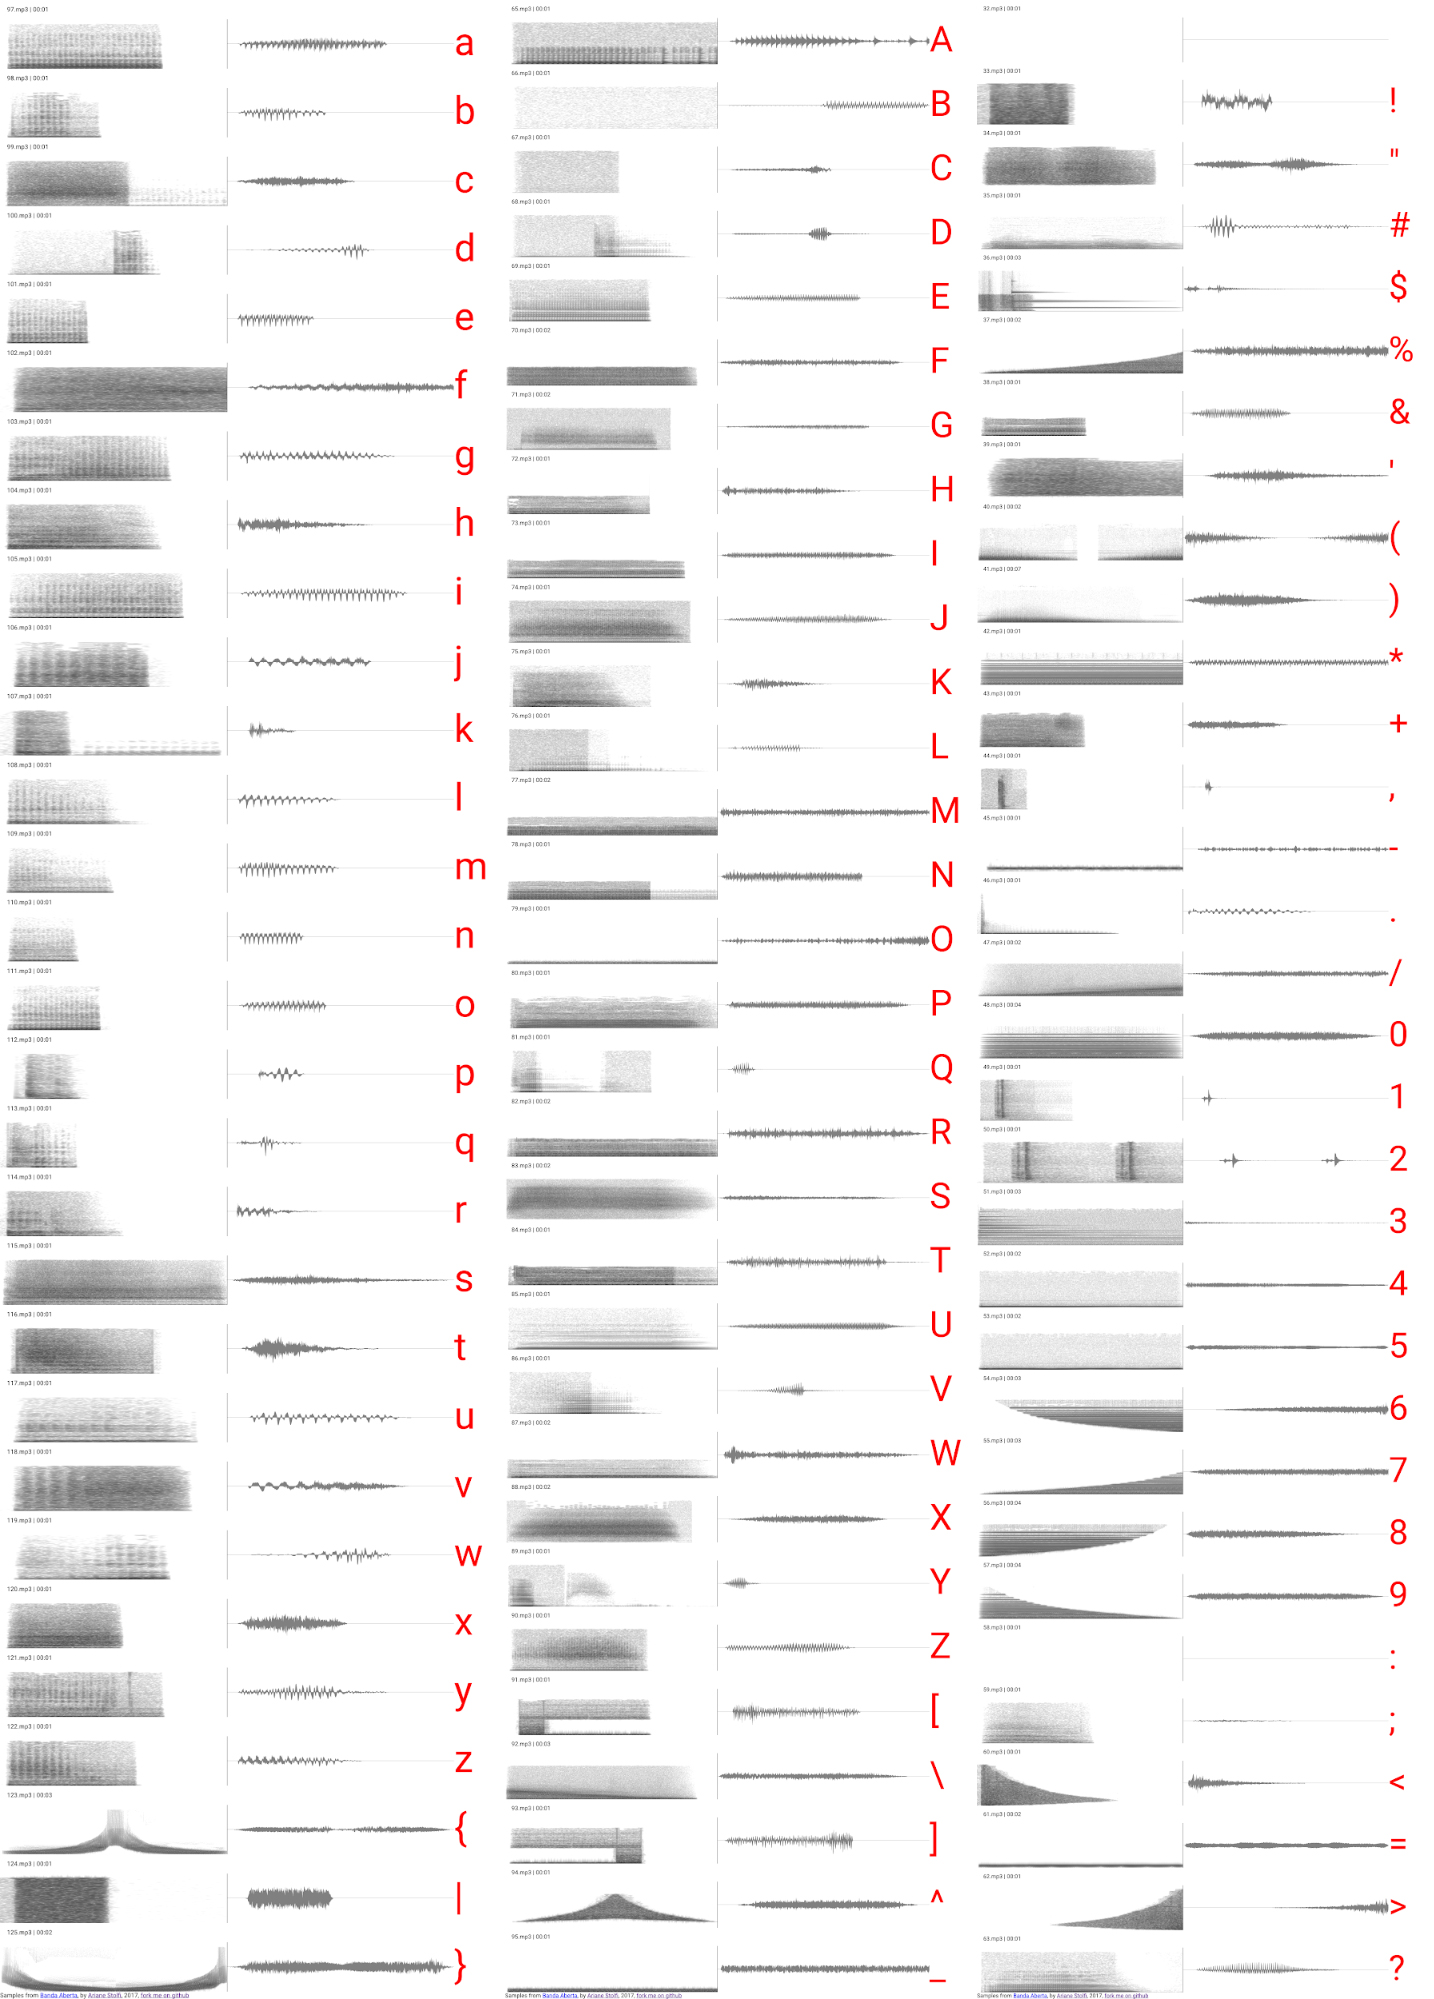
\includegraphics[width=0.7\linewidth]{pictures/cap3/bandagalaxias.jpg}
    \end{center}
    \legend{Fonte: screenshot da autora}
\end{figure}


\item[Percussão e Acordes] Para o segundo conjunto de samples, procurei lidar com materiais mais tradicionais do repertório da música popular eletrônica, como samples de percussão e acordes de sintetizadores extraídos de bancos de samples. Para manter uma estrutura lógica coerente na relação entre sons e letras, sons percussivos foram empregados no papel de articulação (nas consoantes) e acordes de sons contínuos como suporte (nas vogais). Nesta experiência, usamos uma progressão de Dó maior para a composição dos acordes das vogais, com samples gerados por síntese aditiva, e para as letras maiúsculas utilizamos um timbre com mais harmônicos do que os das letras em caixa baixa. \footnote{Exemplos deste pacote podem ser ouvidos em: \url{http://spectro.codigo.xyz/spectrogramplayer/perc.html} }
A associação entre as consoantes e os sons percussivos foi feita através de uma escuta reduzida de uma coleção grande de samples, buscando identificar sons que lembrassem características fonéticas das letras originais, como um bumbo para a letra ``B'' e pratos para ``S''. Mais uma vez aqui, fizemos essa associação mais direta entre sons e fonemas nos caracteres do alfabeto, enquanto para os caracteres especiais procuramos outras relações, como por exemplo entre sua forma visual e o desenho espectral dos sons. Alguns caracteres especiais foram extraídos da peça de Velimir Khleibnikov ``Radio of the Future''\footnote{Disponível em: \url{http://www.ubu.com/sound/russian_avant.html}}.

\begin{figure}[htb]
    \caption{\label{samplespercussao}Espectrogramas do Conjunto de Samples Percussão e Acordes}
    \begin{center}
        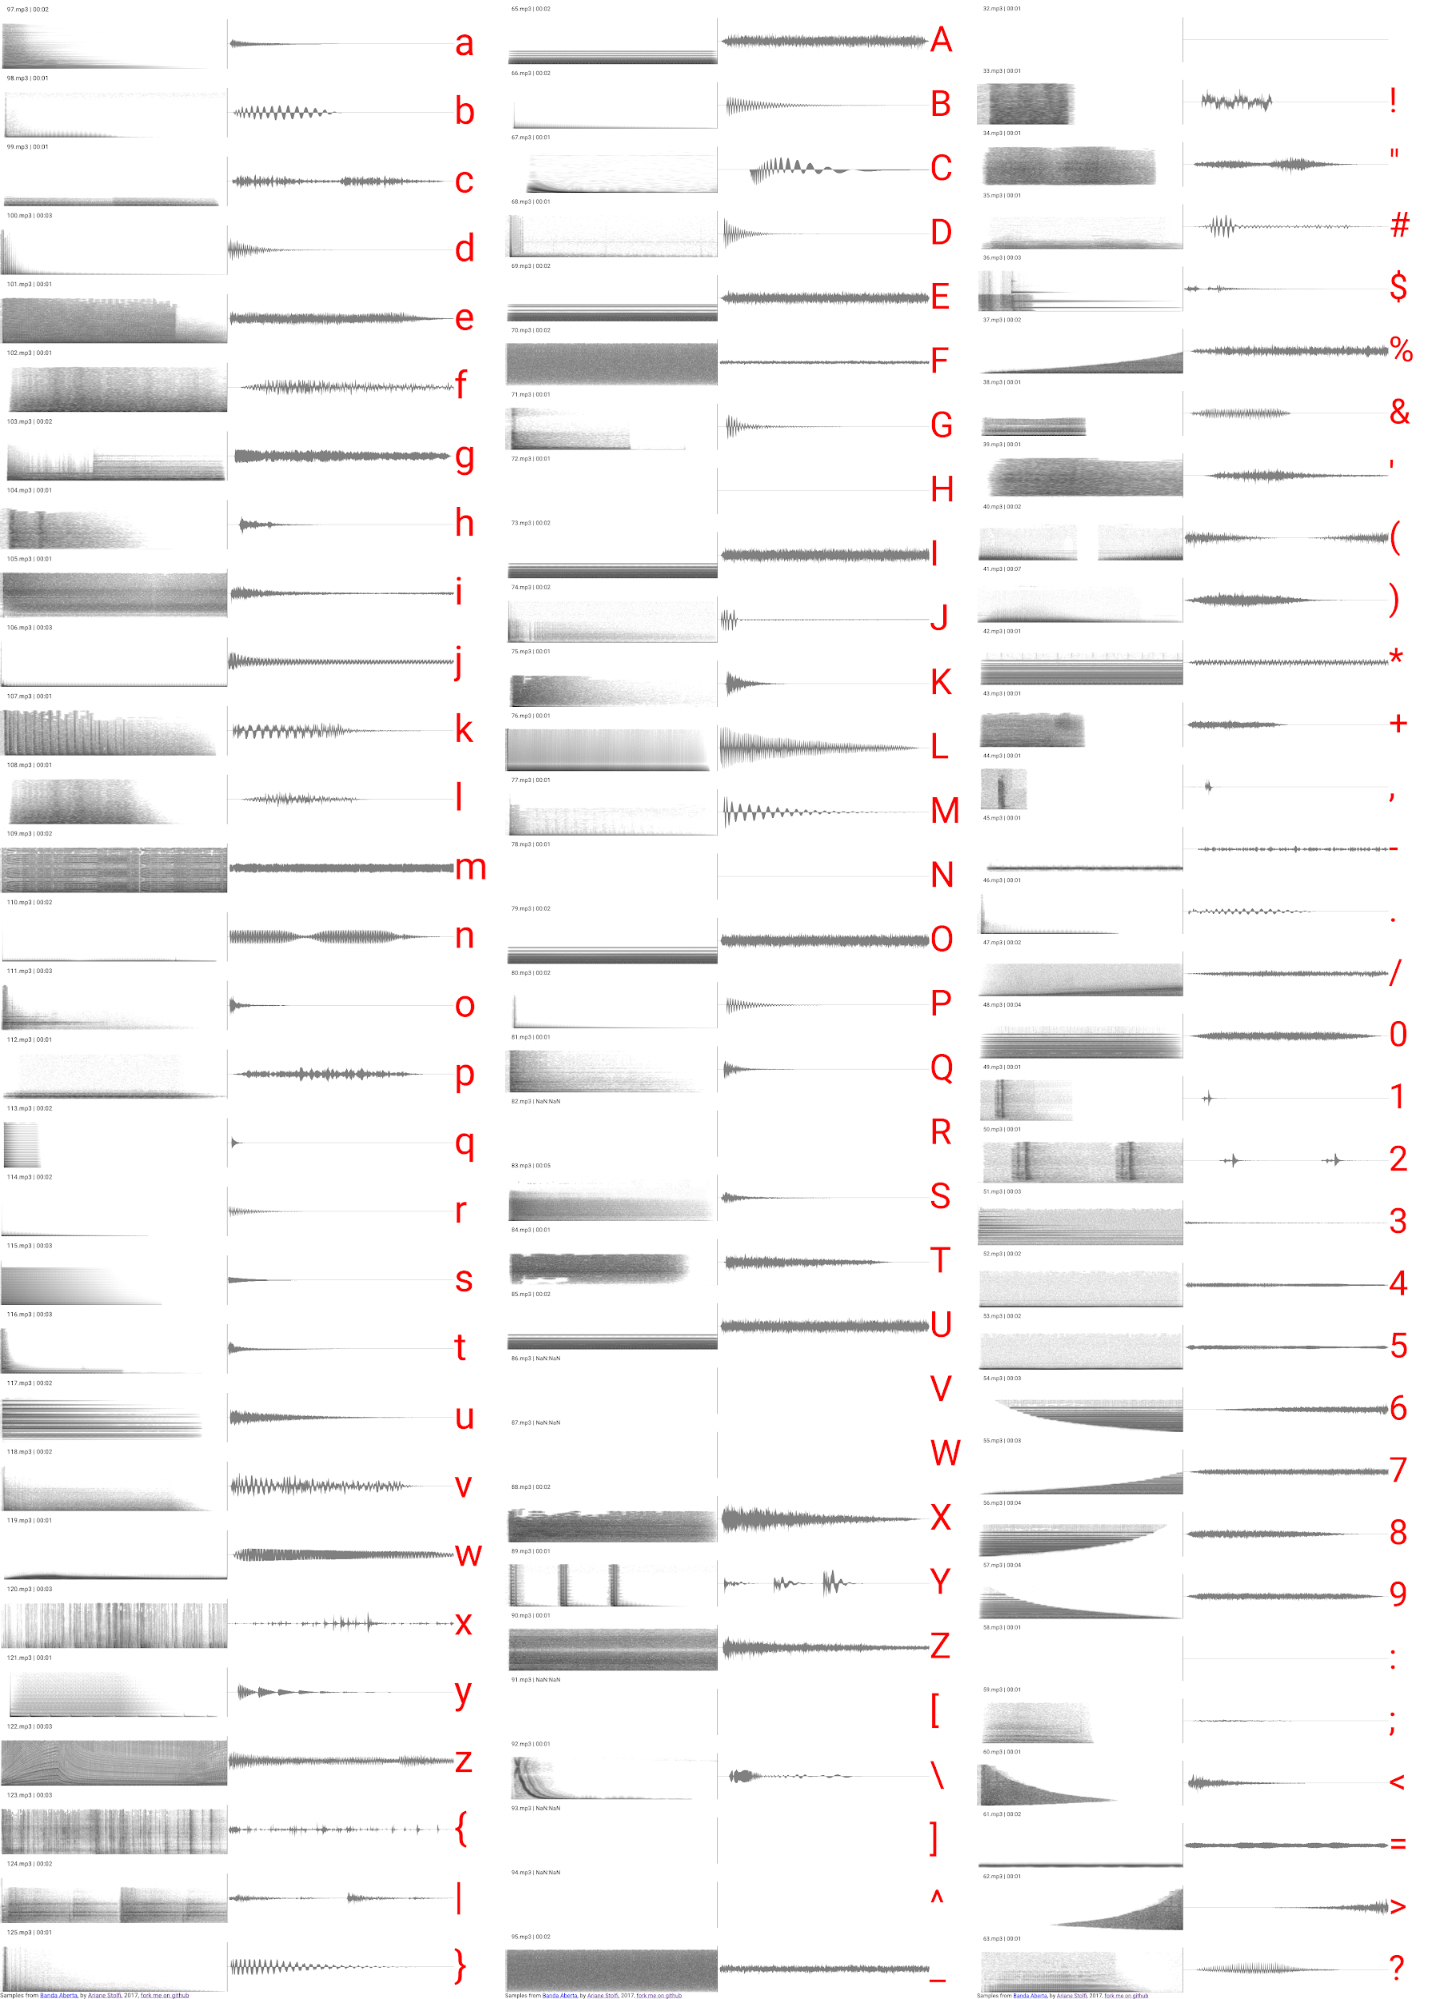
\includegraphics[width=0.7\linewidth]{pictures/cap3/bandapercussao.jpg}
    \end{center}
    \legend{Fonte: screenshot da autora}
\end{figure}

\item[Pacote Colaborativo]O terceiro conjunto de samples foi montado a partir da colaboração de alunos da turma de Produção Musical da Universidade Anhembi Morumbi, sob orientação do professor Viktor Kisil, que solicitou da turma samples para a composição deste conjunto de sons. Este pacote contém samples de fontes sonoras muito variadas, de concretos a sintetizados. A associação entre letras e sons não foi feita procurando analogias como nos outros conjuntos, e sendo assim, ele provém sons mais excêntricos. \footnote{Exemplos podem ser ouvidos em: \url{http://spectro.codigo.xyz/spectrogramplayer/fx.html}} 

\begin{figure}[htb]
    \caption{\label{samplescolab}Espectrogramas do Conjunto de Samples Colaborativo}
    \begin{center}
        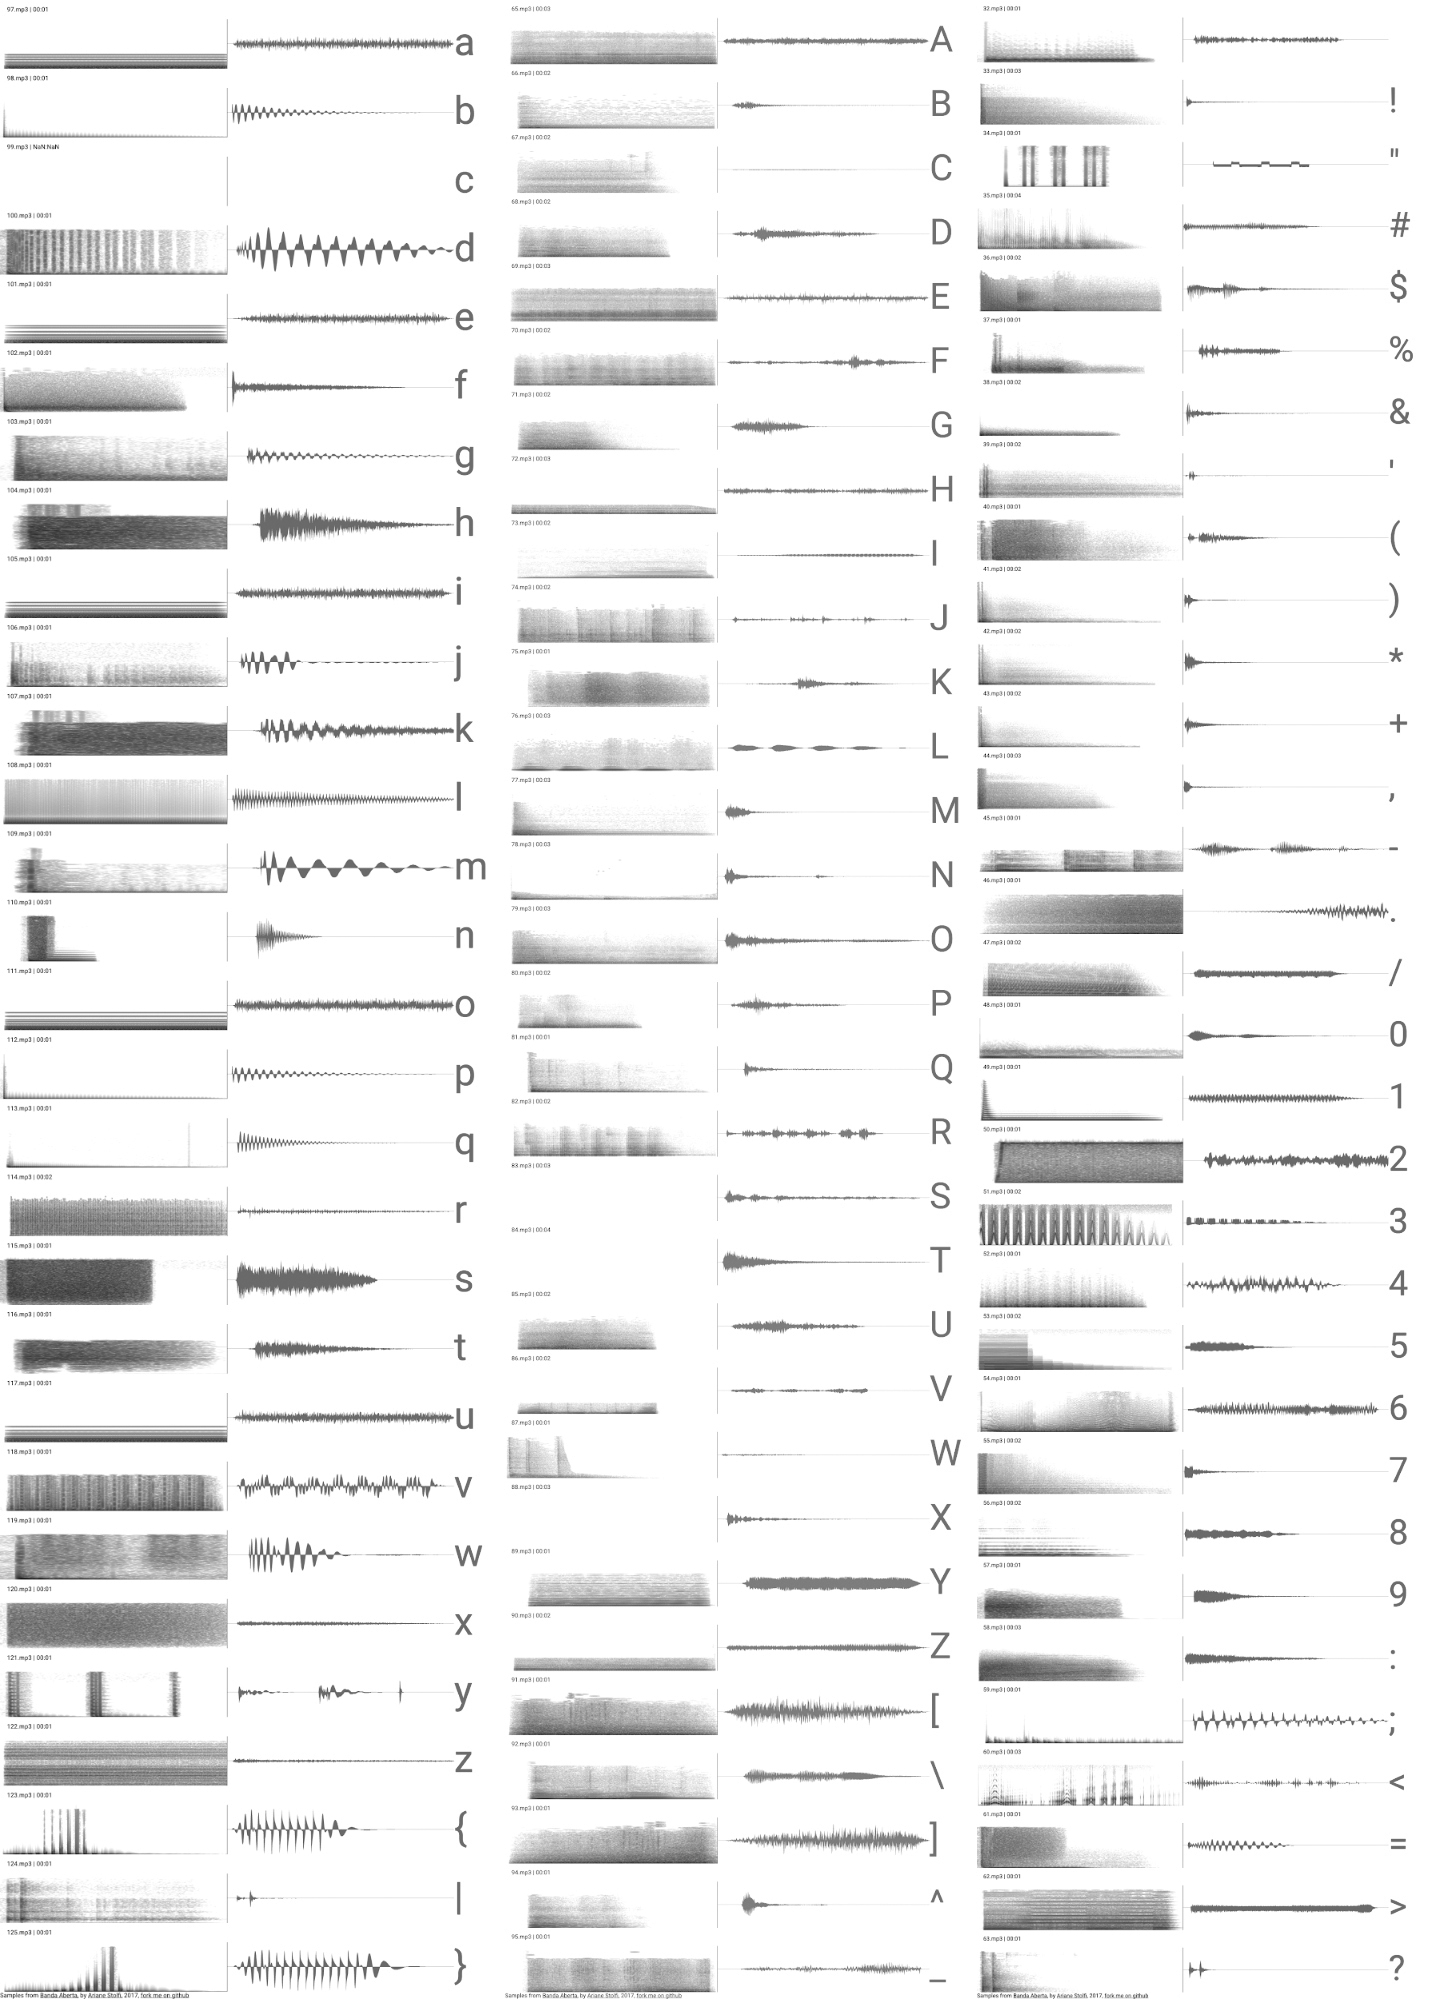
\includegraphics[width=0.7\linewidth]{pictures/cap3/bandaabertacolab.jpg}
    \end{center}
    \legend{Fonte: screenshot da autora}
\end{figure}

\item[Orquestra Errante] O quarto conjunto é formado por samples recortados de gravações de sessões de improvisação musical da Orquestra Errante, conduzida pelo professor Rogério Costa. Eles foram produzidos em sua maioria por instrumentos acústicos, como saxofone, flauta, piano, trombone, contrabaixo, percussão e voz. As gravações base que utilizei foram feitas durante ensaios da orquestra no estúdio do CMU, muitas vezes utilizando técnicas estendidas. Nós obtivemos um arquivo com várias gravações passadas desses ensaios, e empregamos técnicas de escuta reduzida e análise espectrográfica pra identificar ``clangs" que pudessem ser isolados para funcionar como átomos. Aqui novamente aplicamos uma analogia entre os fonemas e os sons sampleados e as funções de articulação para as consoantes e de suporte para as vogais. Para os numerais, usamos analogia entre batimentos e a quantidade representada. Exemplos deste conjunto podem ser ouvidos em: \url{http://spectro.codigo.xyz/spectrogramplayer/orquestra.html}
\end{description}

\begin{figure}[htb]
    \caption{\label{samplesorquestra}Espectrogramas do Conjunto de Samples Orquestra Errante}
    \begin{center}
        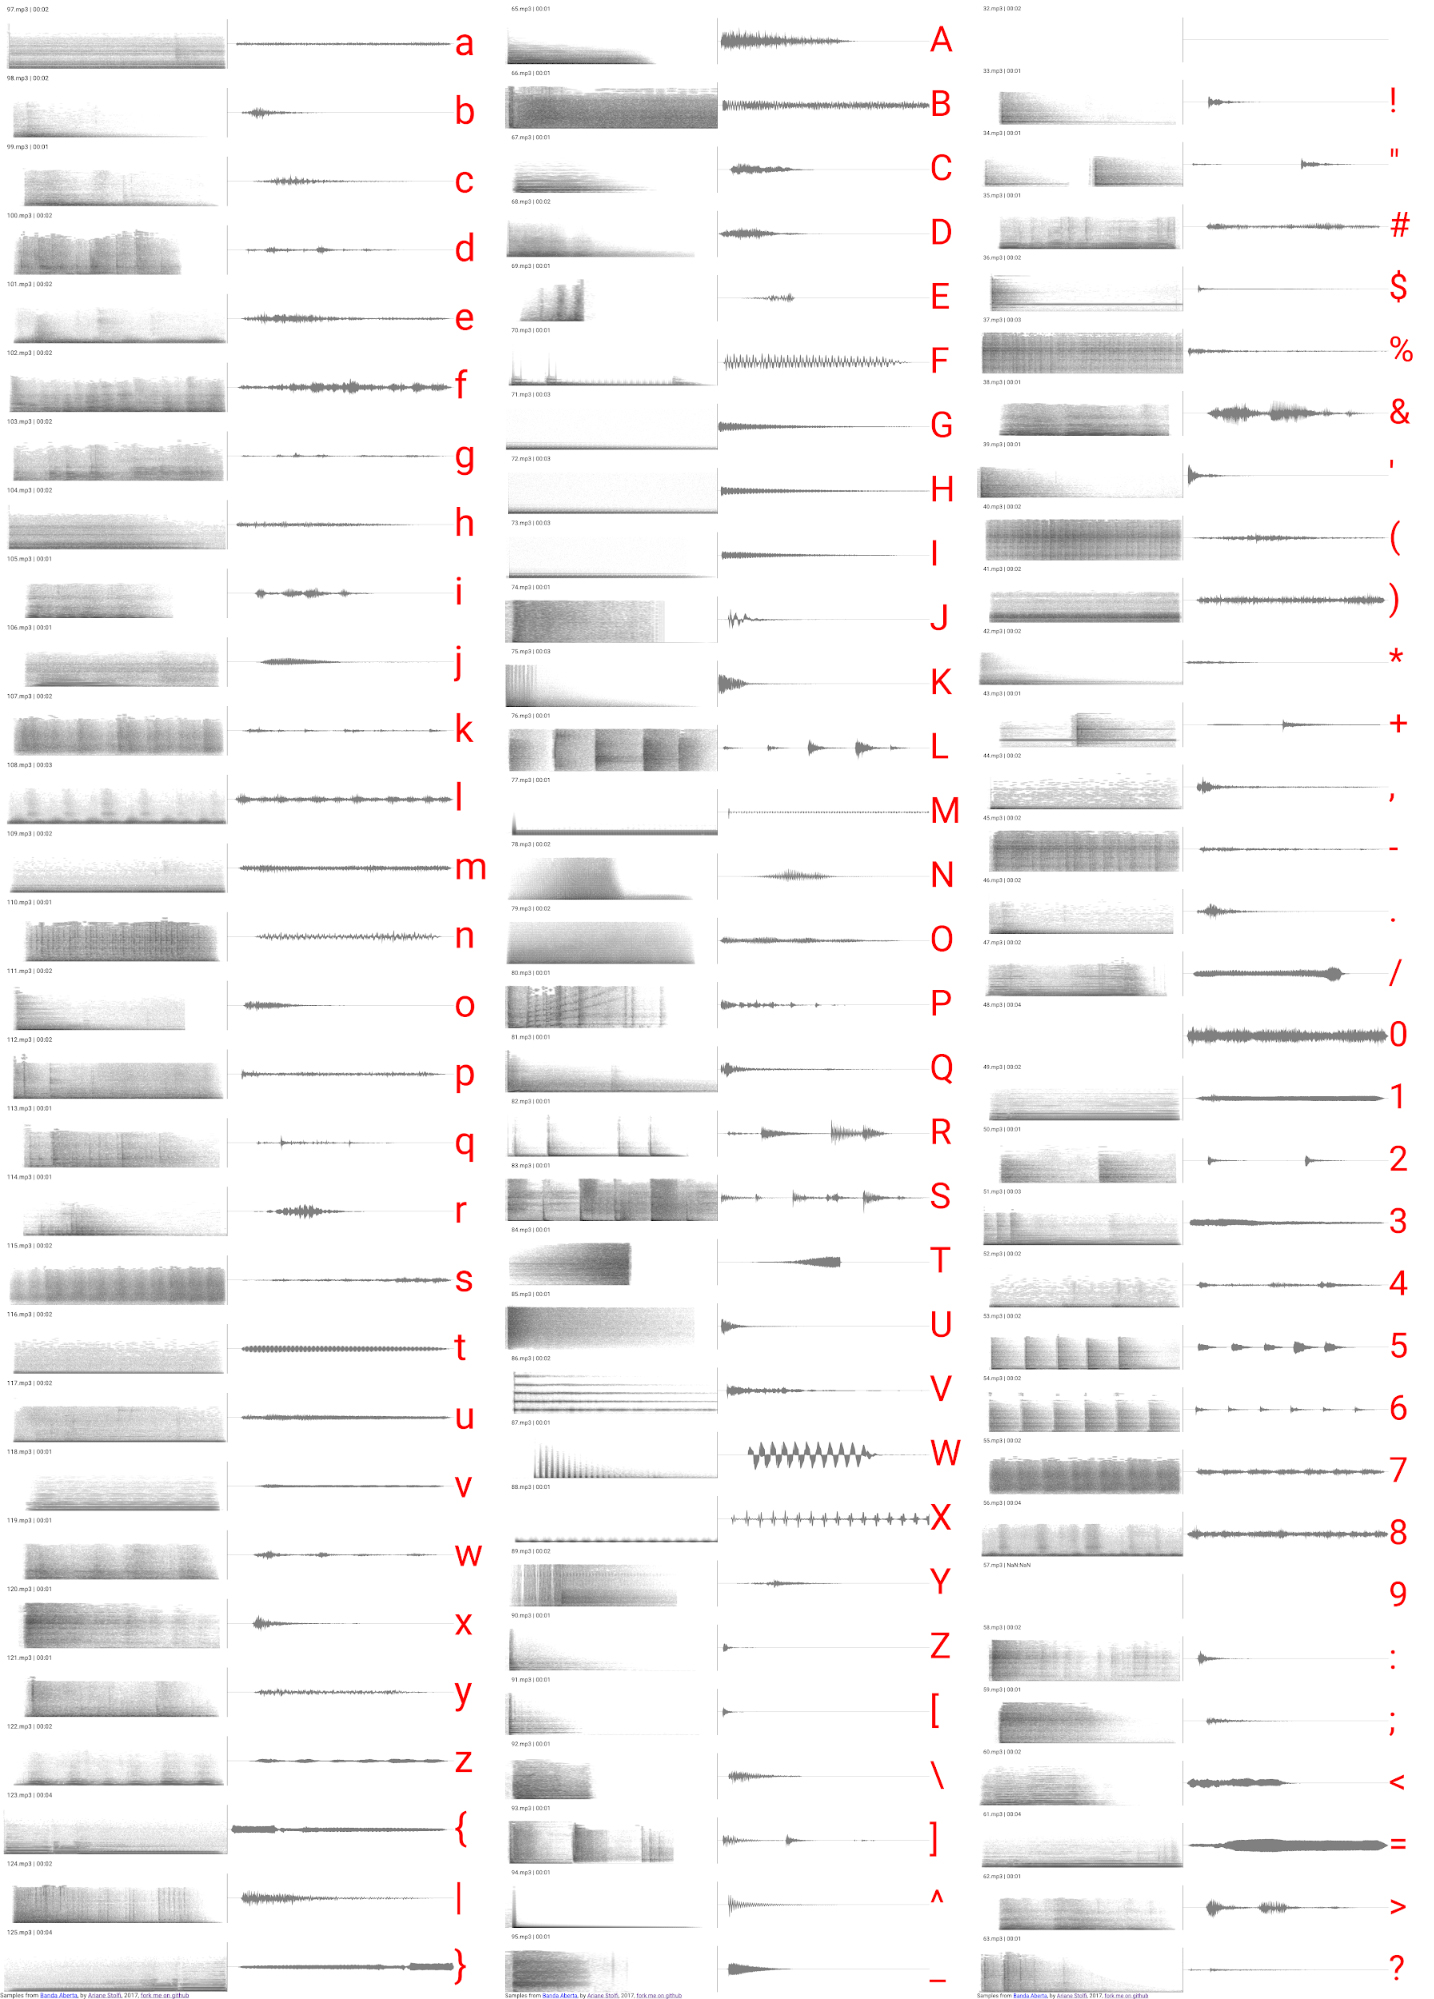
\includegraphics[width=0.7\linewidth]{pictures/cap3/bandaorquestra.jpg}
    \end{center}
    \legend{Fonte: screenshot da autora}
\end{figure}

%It is important to emphasize that the browser used by the participants can make a real difference on the performance itself. Most current browsers do enable web audio synthesis, however they are incompatible with many parameters. That said, the participants are recommended to use Google Chrome and take advantage of its full compatibility with current web audio standards.
\subsection{Segunda Versão: Web Audio Type -- Tipografia sonora}
Em uma segunda versão do projeto \cite{Stolfi2017w}, onde nosso objetivo era testar uma versão totalmente baseada em síntese sonora no browser, procuramos explorar uma abordagem diferente para o processo de tradução intersemiótica. Nesta segunda versão, desenvolvemos um sistema de analogia direta entre as formas das letras e o perfil espectral dos sons gerados, criando um ``alfabeto sonoro'' que ao mesmo tempo em que soava, desenhava a forma do texto no espectro. Para tanto, fizemos uma associação entre osciladores -- que desenhavam as linhas horizontais e as inclinadas -- e um sintetizador de rúido baseado em FFT que foi desenvolvido especialmente para o projeto -- que construía os blocos verticais das letras desse alfabeto sonoro.

Durante o desenvolvimento desta nova versão, nós optamos por avaliar a possibilidade de integração com algumas soluções pré programadas para síntese sonora via web, como os \emph{frameworks} Gibber \cite{Roberts2012gibberlivecoding}, Waax~\cite{Choi2013waax}, e meSpeak.js~\footnote{meSpeak.js website: \url{http://www.masswerk.at/mespeak/}}. Utilizar soluções prontas para síntese sonora poderia faciliar o uso e compatibilidade da tecnologia, mas ao mesmo tempo também criaram certas barreiras e imporiam algumas limitações que não são oferecidas pelo uso de web Audio ``puro''. Além disso, alguns desses frameworks ofereciam muito mais recursos do que o necessário pelo projeto, que poderia dificultar o processo de desenvolvimento. Nós tentamos usar o framework meSpeak como uma ferramenta simples para conversão de texto em discurso, mas o resultado sonoro final não foi musicalmente satisfatório, e ele não permitia que se tocassem mensagens umas em cima das outras. No final, decidimos desenvolver uma solução toda em Web Audio, para a programação do processamento de áudio.



%During the development of this new version we opted to evaluate some ready-made solutions for web audio synthesis like Gibber~\cite{Roberts2012gibberlivecoding}, Waax~\cite{Choi2013waax}, and meSpeak.js~\footnote{meSpeak.js website: \url{http://www.masswerk.at/mespeak/}}.
%These solutions are able to facilitate the use of web audio technology and other browser facilities, but also create barriers and sometimes limitations that weren't imposed by pure web audio. Furthermore, sometimes frameworks could offer more than what was required by the application, which can lead to more confusion during development. We tried to use, meSpeak.js as a simple and interesting text-to-speech library but the resulting sound was not musically satisfactory, and we couldn't make messages play one on top of each other, due to limitations of the framework, so we choose to focus on pure web audio for sound programming.

Após as primeiras experiências com síntese de voz, decidimos por uma outra abordagem estética, baseadas em conceitos de design tipográfico \cite{ruder_typography:_2009} para propor uma ``tipografia sonora'', e também para experimentar com novas formas de fazer música, evitando acordes e escalas tradicionais da música ocidental. Essa idéia guiou toda a proposta de desenvolvimeto dessa nova versão e causou um grande impacto no resultado obtido.

Essa idéia de ``tipografia sonora'' já havia sido explorada em um trabalho anterior que eu desenvolvi em 2014, chamado ``Utopia'', onde trabalhei a com síntese subtrativa a partir de uma base ruidosa, que era a gravação de uma serra de fita em atividade, para desenhar a palavra UTOPIA no espectro sonoro. Nesse caso, bem como na versão em Web Audio do Banda Aberta, nós também partimos de uma idéia de tradução intersemiótica, assim como na outra versão, mas aqui, procuramos uma relação de isomorfia entre o desenho das letras e som, dispensando a relação fonética. Para tanto, projetamos ``letras'' formadas por blocos de sons pré-determinados, através de síntese aditiva e síntese de ruído, para sonificar o desenho das letras do alfabeto.



%We also decided to follow some aesthetic concepts based on type design~\cite{ruder_typography:_2009} to propose ``an audio typograph", and also to experiment with new kind of music, avoiding traditional chords and scales. These concepts surrounded the whole development of this current version of Open Band and had a great impact in the new result obtained.

%In this particular version, we are also using a concept of audio typography as base to this inter-semiotic translation, to decode letters into sounds, building spectral designed ``letters" made of predetermined sound blocks. Trough this path, we are abstracting the aural aspects of the typed characters and grabbing only the shape of the letters as information for the sound synthesis.

%The effect of typography on written texts acted as a motivation in the present artifact to experiment with ways in which timbre could affect the sound produced by musicians. We use additive and noise synthesis to sonify ``drawings" of the shapes of the letters.


\begin{figure}[!ht]
    \centering
        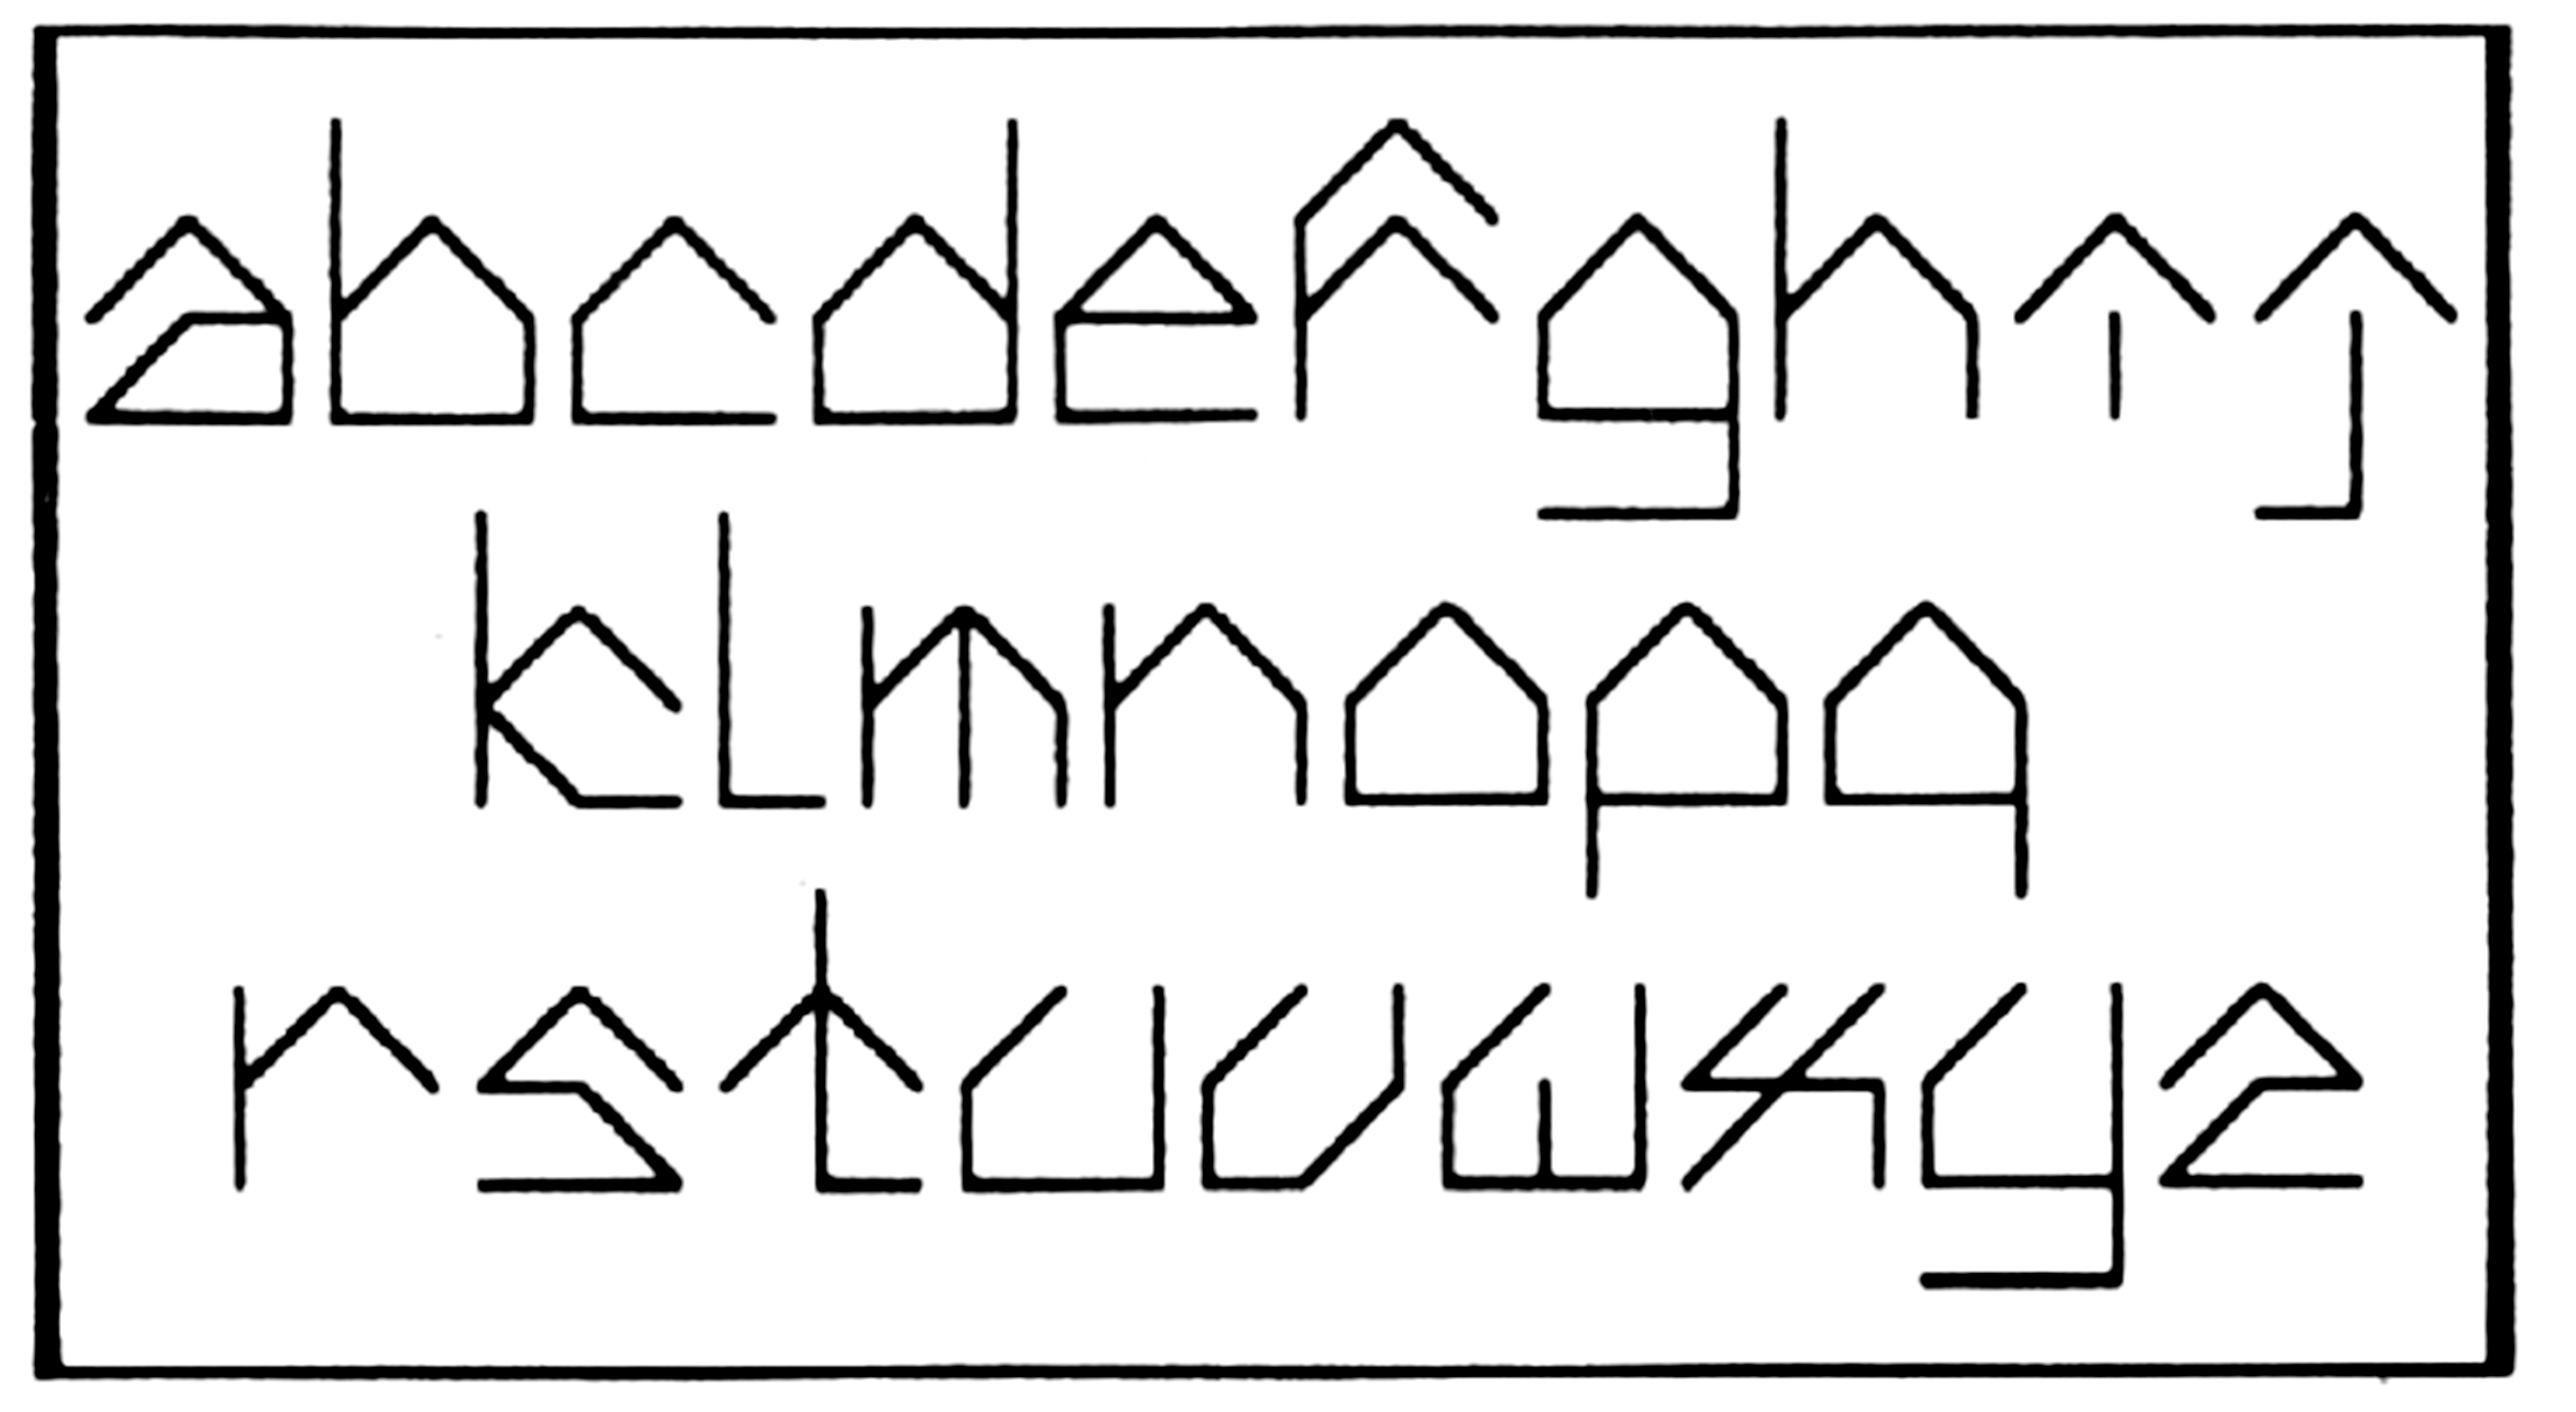
\includegraphics[width=0.8\linewidth]{pictures/metamagical}
        \vspace{-10pt}
    \caption{One of the modular alphabets proposed by Douglas Hoefstader in the book Metamagical Themas, page 90}
    \label{fig:metamagical}
\end{figure} 

Um dos pontos de partida para essa idéia foi o trabalho de Donald Knuth, um cientista da computação que trabalhou com questões de tipografia, e desenvolveu o conceito da ``meta-fonte'', um tipo que não era desenhado estaticamente, mas cujo desenho poderia variar de acordo com parâmetros tipográficos\cite{knuth-meta-font_1982}. A partir do design dessa ``meta-fonte'', muitas famílias tipográficas diferentes poderiam ser geradas, simplesmente pela mudança de parâmetros como: altura, largura, espessura, linha de base, altura de x etc. Como aponta Douglas Hesfstader:

\begin{citacao}
Knuth's purpose is not to give the ultimate parametrization of the letters of the alphabet (indeed, I suspect that he would be the first to laugh at the very notion), but to allow a user to make ``knobbed letters" -- we could call them letter schemas. This means that you can choose for yourself what the variable aspects of a letter are, and then, with Metafont's aid, you can easily construct knobs that allow those aspects to vary. 
(...)
Knuth's purpose is not to give the ultimate parametrization of the letters of the alphabet (indeed, I suspect that he would be the first to laugh at the very notion), but to allow a user to make ``knobbed letters" -- we could call them letter schemas. This means that you can choose for yourself what the variable aspects of a letter are, and then, with Metafont's aid, you can easily construct knobs that allow those aspects to vary~\cite{Metamagical1986}. 
\end{citacao}

%Donald Knuth, a computer scientist and artist who worked on typesetting issues, developed the concept of a ``meta-font", a typeface that was not statically drawn, but that could be changed trough typographical parameters\cite{knuth-meta-font_1982}. Following the rules of meta-fonts, many different typefaces could be generated simply by varying the type parameters. As says Douglas Hoefstader in ~\cite{Metamagical1986}, \textit{``Knuth's purpose is not to give the ultimate parametrization of the letters of the alphabet (indeed, I suspect that he would be the first to laugh at the very notion), but to allow a user to make ``knobbed letters" -- we could call them letter schemas. This means that you can choose for yourself what the variable aspects of a letter are, and then, with Metafont's aid, you can easily construct knobs that allow those aspects to vary."}.





\begin{figure}[!ht]
   \centering
       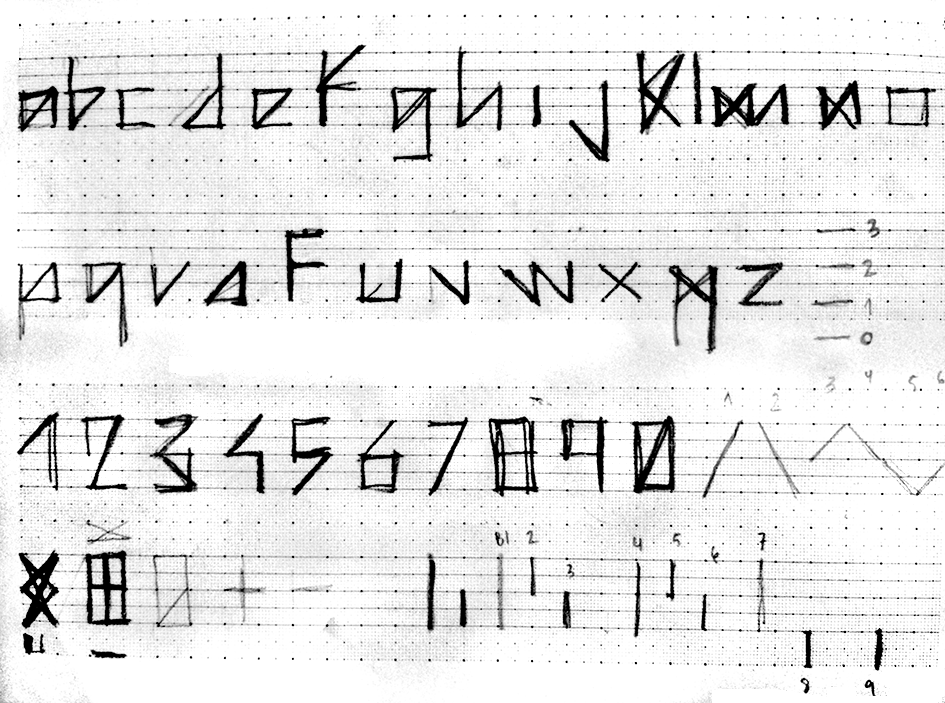
\includegraphics[width=0.8\linewidth]{pictures/audiotype_sketch}
   \caption{Sketch for the modular font to be base for audio synthesis.}
    \label{fig:sketch}
 \end{figure}


%\begin{figure}[!hb]
%   \centering
%       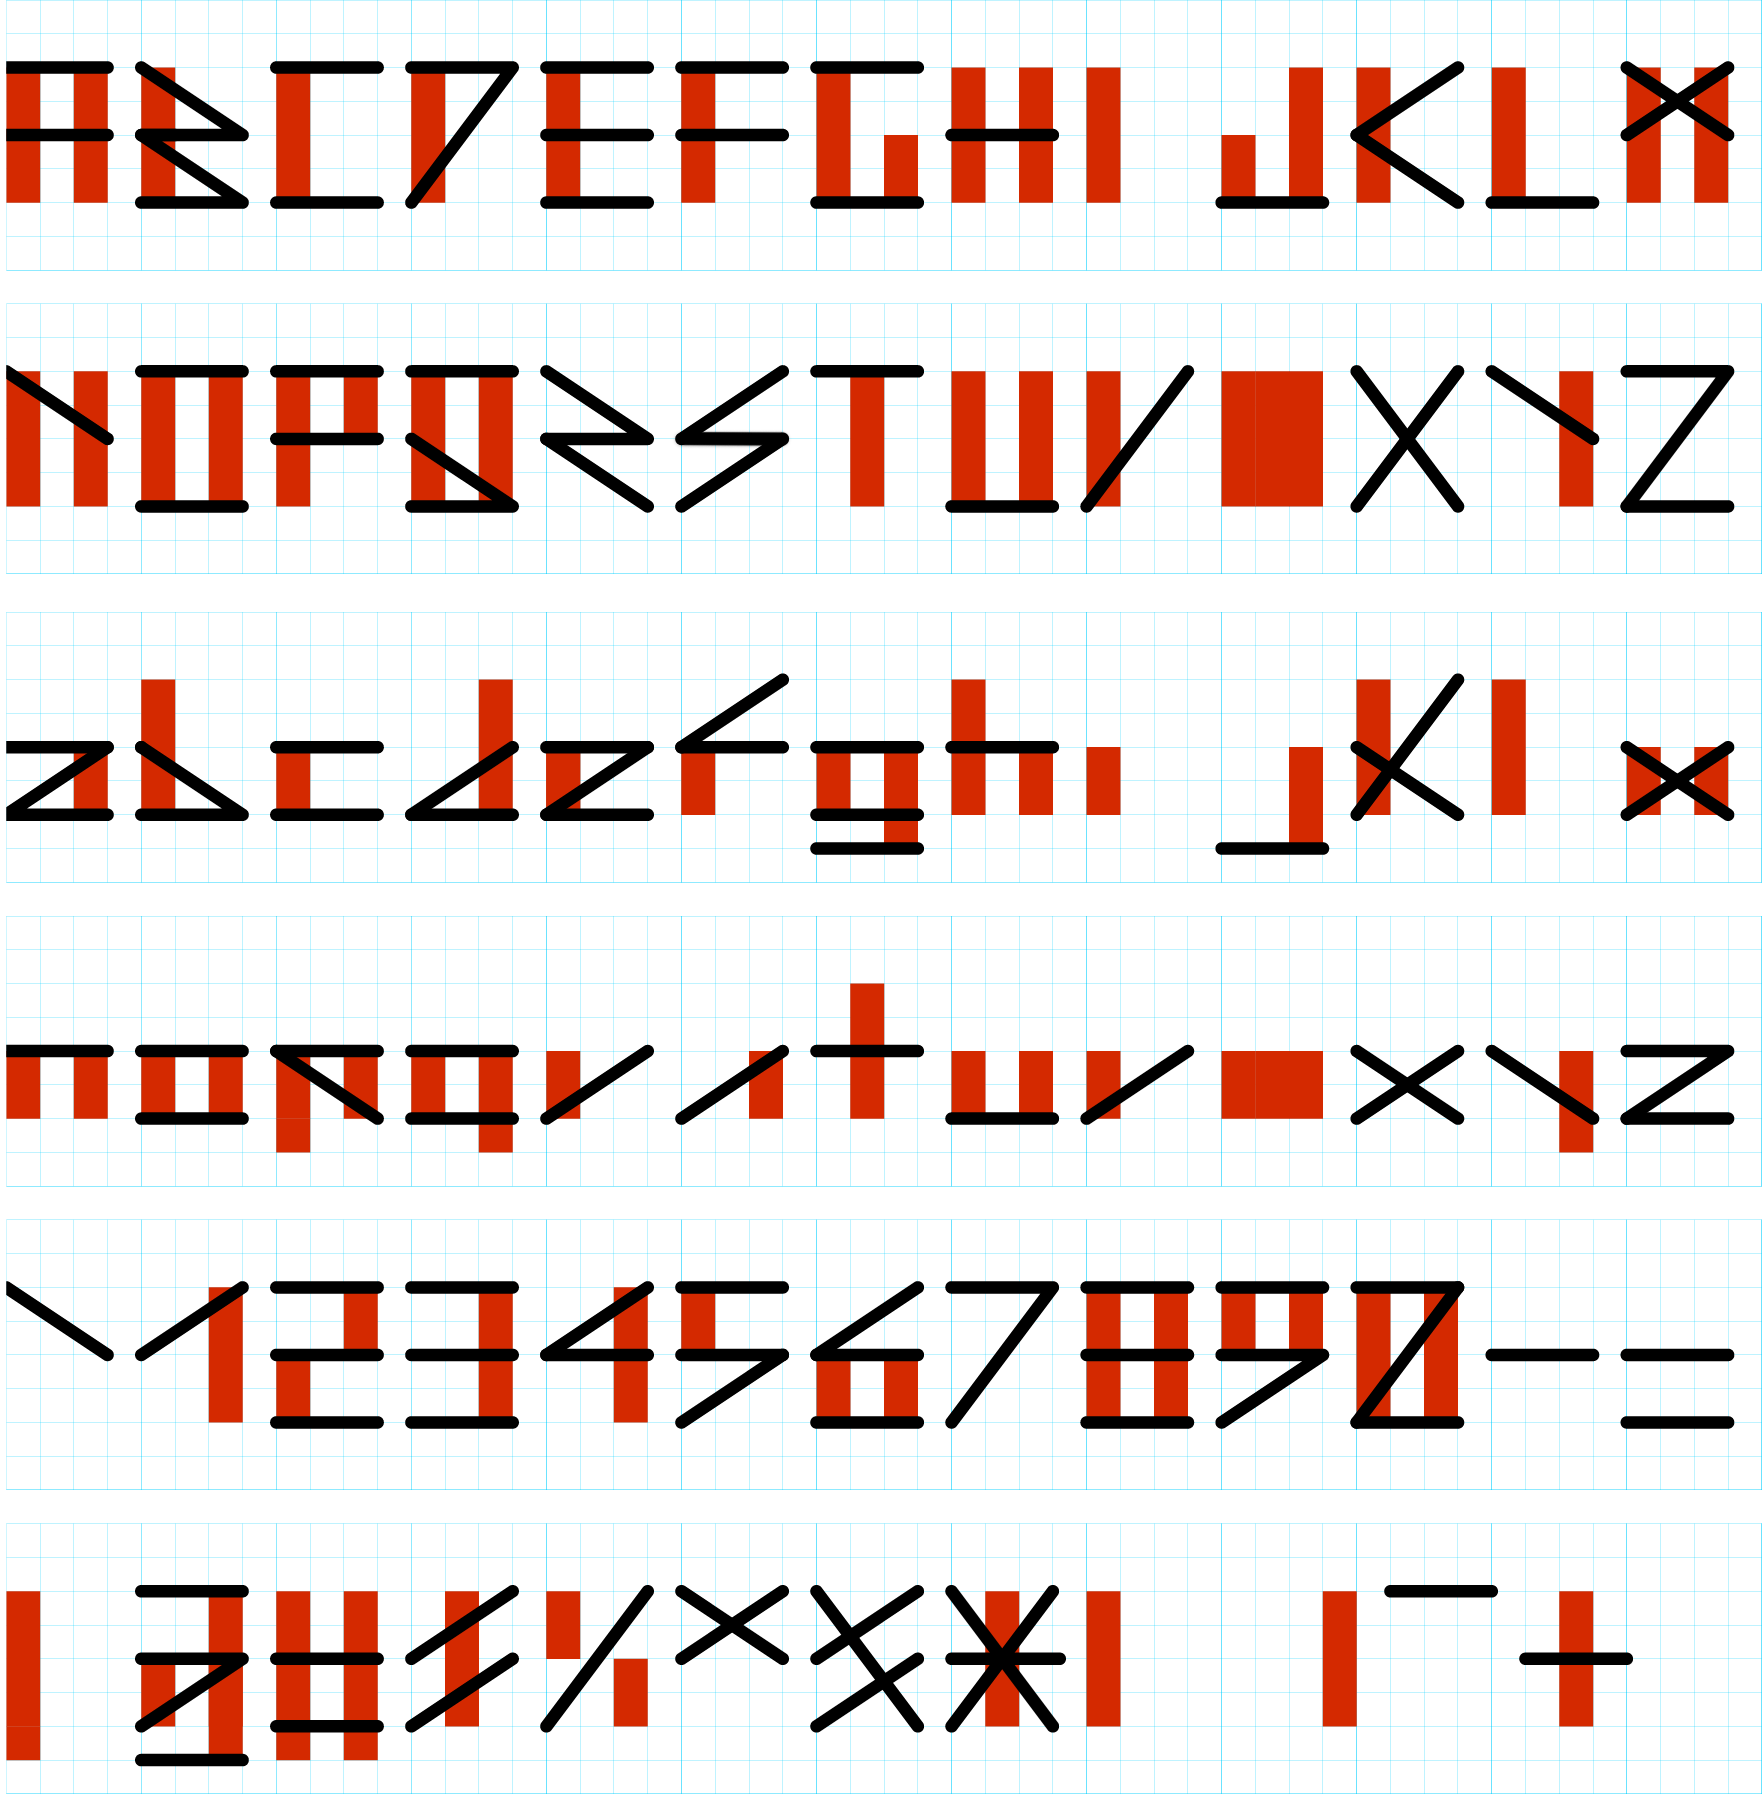
\includegraphics[width=0.45\textwidth]{pictures/audiotype_v1_2_2}
%       \vspace{-10pt}
%   \caption{Project for audio typography, made of blocks of noise, sine waves and glissandi. The red blocks represent noise and the black lines solenoids and glissandi.}
%   \vspace{-10pt}
 %   \label{fig:project}
%\end{figure}

Nós usamos alguns desses parâmetros tipográficos definidos por Knuth para estabelecer frequências geradoras para os sons puros: as frequências mais baixas corresponderiam às linhas dos descendentes, a linha de base para a segunda, a altura de x para a terceira e a altura da caixa para a quarta frequência, em ordem ascendente. Os parâmetros horizontais, por sua vez, foram convertidos em medidas temporais, para determinar a duração dos eventos sonoros e dos intervalos entre as letras.

%We used the basic parameters defined by Knuth~\cite{Metamagical1986} such as x-height, baseline, height of ascendants and descendants, as measures to establish frequencies for tone sounds (one low, one at the baseline, one at the x-height an one at the uppercase line of each letter). The horizontal parameters of the type are translated into temporal measures, to determine duration of the sound events and intervals between the letters.   

A meta-font proposta por Knuth é uma fonte complexa com cerca de 36 parâmetros tipográficos variáveis. Para a nossa ``tipografia sonora'', no entanto, propus uma analogia mais simples, semelhante às propostas por Douglas Hoefstader no seu livro ``Metamagical Themas''\cite{Metamagical1986}(ver Figura \ref{fig:metamagical}), baseada em uma estrutura de grelha. Na nossa proposta, as letras seriam desenhadas a partir de poucos elementos básicos, como no rascunho apresentado na figura \ref{fig:sketch}. As linhas das letras foram mapeadas em dois tipos de funções: síntese de noise (noise())baseada em FFT para os blocos verticais, e senóides (sine()) para as linhas horizontais e diagonais (que soam como glissandos), como pode ser visto nas Figuras \ref{fig:noise} e \ref{fig:sine}. 


%A meta-font is a complex font with several typographic parameters. In this work, we are using a simpler analogy by proposing a modular type, similar to the ones Douglas Hoefstader~\cite{Metamagical1986} proposes in his book ``Metamagical Themas", based on simple grid structures (see Figure \ref{fig:metamagical}). We propose a model that can work only with a few building blocks (see Figure in which they are sketched). The line of the letters was mapped into two basic types of functions: noise synthesis for the verticals and solenoids for the horizontal lines and glissandi, as defined by the composer project in Figure x.


A função ``sine()'' tem um \emph{buffer} de oscilador e podem gerar frequências estáticas ou em rampas lineares, deste modo, geram linhas horizontais ou diagonais no espectro. As funções ``noise()'' geram blocos de ruído que vão de faixas de frequência determinadas. Como processo de programação, definimos 20 funções específicas para cada módulo das letras e cada letra é então formada pelos seus módulos correspondentes. 





%Sine function has one oscillator buffer that can have static frequencies or linearly ramping frequencies. This creates diagonal and horizontal lines in the spectrum. Then, frequencies are defined as the bottom and top limit, some steps are defined in the middle. The length of spectral letters are as well defined. By the end, letters are translated as a group of functions, and the result is played one after another. We built 20 predetermined functions to correspond at each ``type block", and each letter plays as many functions as are determined by the typeface project. Thus, we created a system of mapping letters to the functions.

Cada nó de saída de áudio passa também por um envelope ADSR \cite{Lee2016} para gerar uma forma mais natural de ataque e release, e também passa por um nó de ganho que pode ser controlado durante a performance. A figura \ref{fig:spectro}, mostra um espectrograma gerado pelo sistema com os resultados obtidos.

%Every output node goes through an ADSR class \cite{Lee2016} that creates a more natural attack/release, and also goes through a gain node, that can be changed during a performance. On Figure \ref{fig:spectro} is shown a spectrogram generated by the application with the results obtained.

\begin{figure}[!ht]
    \centering
        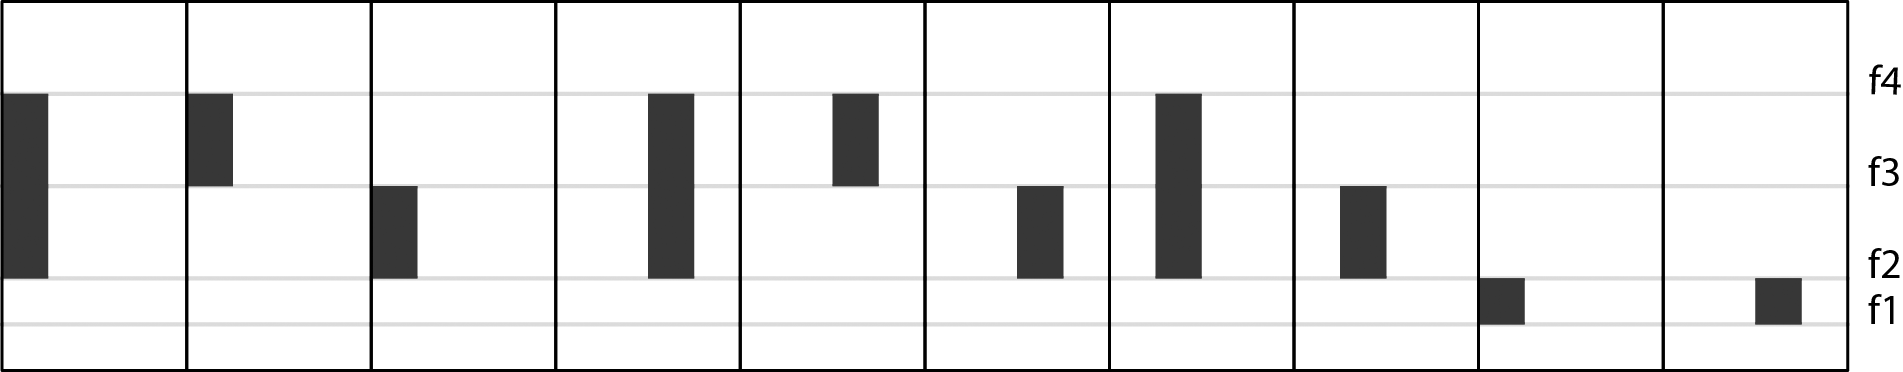
\includegraphics[width=1\textwidth]{pictures/audiotype_v1_noise}
        \vspace{-10pt}
    \caption{Functions for playing vertical blocks with noise synthesis}
    \vspace{10pt}
    \label{fig:noise}
        \centering
        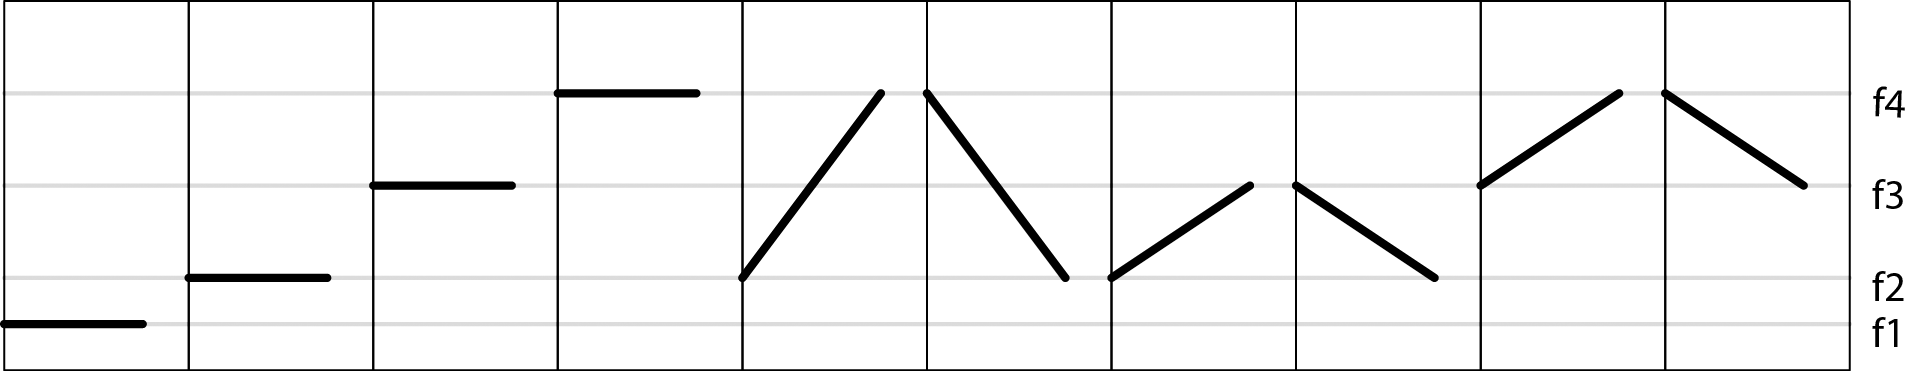
\includegraphics[width=1\textwidth]{pictures/audiotype_v1_sine}
    \caption{Functions for playing horizontal and diagonal lines with oscillators}
    \vspace{-10pt}
    \label{fig:sine}
\vspace{10pt}
\end{figure}

\begin{figure}[!ht]
    \centering
        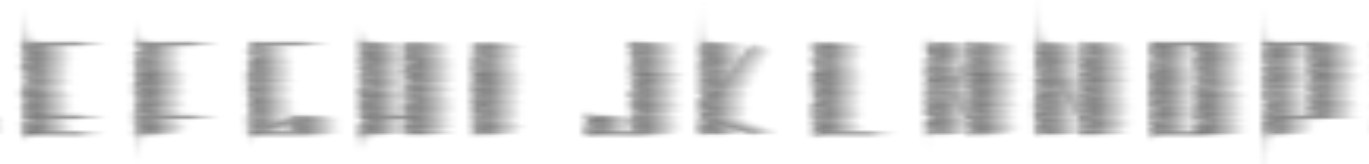
\includegraphics[width=1\textwidth]{pictures/spectrogram}
        \vspace{-10pt}
    \caption{Spectrograms generated by the application}
    \vspace{-10pt}
    \label{fig:spectro}
\end{figure}

%As every letter from every message is translated into a group of playing Web Audio nodes, the number of oscillators that plays simultaneously can grow really quickly depending on the number of participants sending messages. As this application was intended to play in many different mobile devices, this led to the necessity of limiting the creation of nodes, as this could take more processing than some devices could take, and in some cases could make the device stop playing, which is undesirable behavior for such application.






\subsection{Apresentações públicas}
Nós apresentamos o Banda aberta em diferentes ocasiões, para diferentes perfis de público. Dependendo do perfil dos participantes, a conversa foi para direções diferentes. Em uma primeira fase, apresentamos o projeto rodando em um servidor local, que era acessado através do endereço IP, para reduzir a latência e manter o público reunido em uma mesma rede. Posteriormente, passamos a usar a versão online do sistema em outras performances, para facilitar o processo de montagem. Até o momento, realizamos as performance seguintes:

\begin{description}

\item[Ensaio no Nusom] 
A primeira apresentação informal do projeto aconteceu na reunião do NuSom do dia 9 de maio de 2016. O público presente era de pesquisadores do grupo, e cerca de 9 pessoas participaram da experiência. Notamos uma diferença considerável de tocabilidade entre quem estava com laptop em relação a quem estava com celulares. O site também não funcionava em todos celulares, especialmente modelos de iphone mais antigos. \footnote{Registro da apresentação em \url{https://www.youtube.com/watch?v=Utc_4mT5b8s}}

\item[Festival Bigorna]
No dia 26 de junho de 2016, estreamos publicamente o projeto no Festival Bigorna, que aconteceu na Praça José Molina, próxima à Avenida Paulista em São Paulo. O Estúdio Fita Crepe, um pequeno espaço dedicado à produção e difusão de música experimental organizou o festival que ocupava essa praça considerada subutilizada, pela sua localização\footnote{A programação do festival está disponível em: \url{http://www.festivalbigorna.com/2016/}}.

\begin{figure}[!ht]
    \centering
        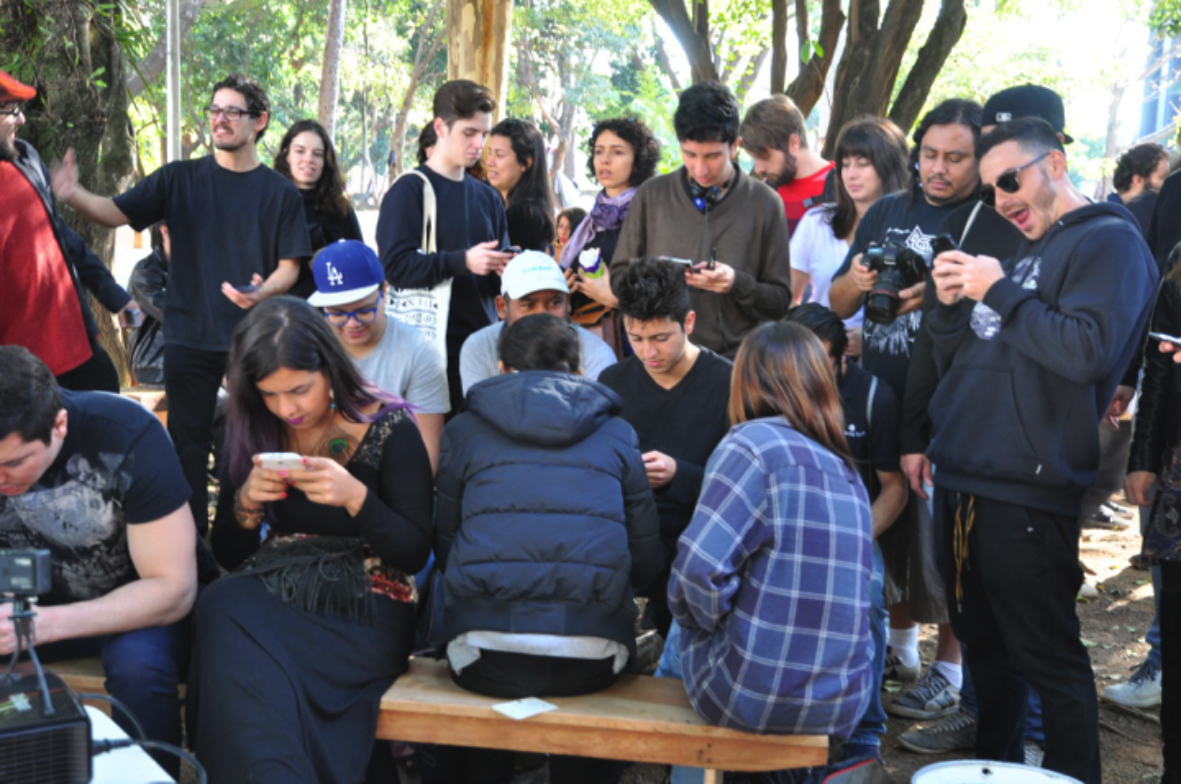
\includegraphics[width=1\textwidth]{pictures/bigorna}
        \vspace{-10pt}
    \caption{people interacting within the piece}
    \label{fig:performer}
\end{figure}

O público presente no momento era de cerca de 80 pessoas, mais do que o roteador podia comportar (30 pessoas ao mesmo tempo), o que deixou várias pessoas de fora da interação. A audiência incluía membros do NuSom, músicos da cena experimental e o público geral do festival, mas grande parte era formada pelos estudantes de produção musical que colaboraram com o terceiro conjunto de samples. Jovens, ficaram bastante eufóricos com a possibilidade do anonimato e praticaram um certo nível de \emph{bulling} entre eles. 

\item[Rádio grave] 30 - 6 -2016
Fomos fazer uma performance também na Rádio Grave, uma rádio web que foi montada no Gfau para ajudar na mobilização dos  estudantes durante a greve do ano passado. Os locutores simulavam que rádio era uma nave espacial, e a ``aterrissagem'' do Banda Aberta por lá rendeu um episódio que ficou conhecido como ``reset do universo'', pela surpresa gerada pelos sons fora do comum. Uma gravação do áudio da performance pode ser ouvido no seguinte link: https://soundcloud.com/asss/banda-aberta-na-radiograve-reset-do-universo.


\item[¿Musica? 12]
No festival, que faz parte de uma série organizada pelo NuSom, apresentamos pela primeira vez a segunda versão do projeto, com síntese sonora em Web Audio, para um público formado principalmente por alunos e professores da Música. 
\url{https://www.youtube.com/watch?v=hRELFhQm6M0&t=639s}


\item[Web Audio Conference] 


\item[Female Laptop Orchestra]
Na performance ``Trasnmusiking'', realizada pelo grupo Female Laptop Orchestra, utilizamos o projeto Banda Aberta em uma apresentação realizada em Londres durante a conferência ``Audio Mostly'' de 2017. A peça contou com a participação remota de 12 pessas, que mandavam streams de áudio de lugares diferentes do globo, esses streams eram mixados em tempo real por Anna Xambó. Além disso, utilizamos o Banda aberta em uma versão com síntese por web Audio, mas somente de ruído, para receber feedback em tempo real da audiência, e também performei com técnicas vocais estendidas e percussão. A audiência era formada principalmente por participantes da conferência, em sua maioria acadêmicos da área de tecnologia musical. A audiência utilizou o chat para dar opiniões sobre a performance e também para piadas com membros da equipe, principalmente Alo, que era um dos organizadores da parte musical.


\item[Audio Mostly Workshop]
Durante o workshop Sounds in the Cloud, organizado em um trabalho conjunto pela equipe do projeto Audio Commons da Queen Mary University of London (QMUL) e pela equipe de pesquisadores do sistema de \emph{Machine Learning} RapidMix da Universidade Golsdmith, os participantes foram convidados a explorar ferramentas desenvolvidas pelos pesquisadores em grupos. Nossa equipe desenvolveu uma versão do projeto Banda Aberta que utilizava a ferramenta RapidMix para mudar parâmetros sonoros através da captura de movimentos pela câmera. Com isso, era possível treinar o sistema para reconhecer certos movimentos em tempo real. Com a experiência, foi possível verificar tanto a facilidade de adaptação do nosso sistema para incorporar tecnologias ded terceiros, quanto a facilidade de utilização do sistema RapidMix para ser incorporado em demais projetos de interação através de sua API em JavaScript.

\item[Encontro da rede de Tecnoxamanismo] 12-8-2016
O encontro da Rede de Tecnoxamanismo na Dinamarca aconteceu na cidade de Aarhus, no ``Dome of visions'', um domo geodésico na região portuária da cidade, onde acontecem uma série de eventos ligados à sustentabilidade, agroecologia, ecologia e temas afins. Além de colaborar na produção do Evento, apresentei a performance para um público que incuía músicos, produtores, performers e interessados de uma maneira geral. O público foi muito comportado no sentido de não escrever muitas bobagens no chat. Nesta performance, utilizamos a versão online da ferramenta, sem o servidor local.


\item[SHA Festival] 7-8-2017
O Festival ``Still Hacking Anyway'' é um encontro de hacker, programadores, pensadores e ativistas que acontece de quatro em quatro anos na Europa. Na edição de 2017 do evento, apresentamos o projeto em uma performance de 45 minutos, onde participaram interessados de diversas partes do mundo. Por ser um festival hacker, a maior parte do público portava laptops ao invés de celulares, o que permitiu uma maior agilidade na digitação das mensagens. Alguns dos presentes passaram a performance tentando hackear com o intuito de derrubar o sistema, o que ocorreu a cerca de 40 minutos depois do início, através de um script que sobrecarregou o sistema e causou uma pane no audio buffer. Pelas características do evento, que era um festival hacker,  já esperávamos um comportamento deste tipo por parte da audiência, que ocorreu até mais devagar do que o esperado. O ataque, no entanto, não causou nenhum tipo de dano ao servidor, que voltou ao normal logo que a performance se encerrou.

\item[aMostra Sonora] 2-7-2016
Na apresentação que fiz solo no festival aMostra Sonora em 2016, utilizei um patch de Pure Data que venho desenvolvendo desde 2006, chamado Modulari, que se baseia em samplers, sintetizadores por \emph{waveshaping}, efeitos para o microfone e osciladores, em conjunto com o Banda aberta. Durante a performance, que durou 40 minutos, utilizei os dois sistemas e técnicas vocais expandidas em conjunto. Apesar de ter corrido normalmente, considerei que os resultados sonoros do conjunto ainda eram limitados, na possibilidade de variação sonora, e passei a planejar um sistema alternativo que fosse mais rico também para performances solo, que descreverei na próxima seção desta tese.




\item[Congresso da Abrapem]

No congresso da Associação Brasileira de Performance musical (30 de junho de 2016), o público de cerca de 23 pessoas, era majoritariamente formado por músicos tradicionais, que ficaram perguntando sobre as referências musicais, de onde vieram os samples, e experimentaram bastante com possibilidades rítmicas. Um registro da performance pode ser visto em:  \url{https://www.youtube.com/watch?v=NOWapLq6eiU}.



\item[Concerto de Computação Musical no IME] (22-9-2016)
No concerto de computação musical no IME aconteceu uma coisa inusitada, o público era formado majoritariamente por programadores e um dos participantes percebeu que era possível inserir comandos em HTML e CSS através do chat. Logo, os participantes começaram a encher a tela com formas geométricas e letras em movimento, e ficaram eufóricos com essa possibilidades de hackear o chat. A gravação da tela da apresentação pode ser vista em: https://www.youtube.com/watch?v=xs23z1IfPfY. A facilidade de uso levou a um grande engajamento do público durante as performances, e traz também um grande nível de divertimento, aproximando assim, como desejávamos, atividade musical de um contexto mais lúdico como o de jogo.

\item[Áudio Insurgência] (7-10-2016)

No festival Áudio insurgência (8 de outubro de 2016), o público era formado principalmente por membros e entusiastas da cena de música experimental e noise de São Paulo. A mesa de som da casa estava com defeito, então ligamos ligamos o celular diretamente nas caixas de som. Também não havia projeção, então não se estabeleceu um ponto focal, e as pessoas ocuparam todos os espaços da casa com seus dispositivos. A gravação do chat pode ser vista em: https://www.youtube.com/watch?v=DpCuU41tWM8 

\end{description}







\section{Análise preliminar}

%comment: In section 4, the authors allude to issues of cross-browser compatibility, but in 3.3.8 they suggest it "is working correctly" on all major browsers. This seeming contradiction needs to be resolved, and hopefully in a way that explains in more detail the issues encountered, the solutions, and any broader take-aways in terms of the future of web audio API.

Em uma análise inicial, foi perceptível que em contextos onde a audiência tinha mais relação com o meio musical, havia uma tendência maior dos participantes passarem mais tempo experimentando com os sons e com o ritmo, digitando mensagens sem significado discursivo. Quando o público era mais jovem, os participantes tendiam a jogar mais com a possibilidade de escrever anonimamente. Quando as conversações começavam a esquentas, camadas de sons eram sobrepostas, tornando o ritmo mais frenético.

Como em uma conversa real, se as pessoas não param para ouvir uns aos outros, a comunicação se torna mais confusa. Nós recebemos através do chat, durante as performances, uma boa quantidade de \emph{feedback} dos usuários, com pessoas perguntando tanto sobre o sistema quanto sobre os sons, e elogiando a performance.

%We observed that in musical contexts, the audience keeps more time experiencing with the samples and rhythm, typing meaningless phrases, and when the public is younger, the participants tend to play with the ability to speak anonymously. 
%As the conversation ``warms" up, layers of sounds are overlapped, turning the rhythm into something more frenetic. 

%Like in a real conversation, if people don't take time to listen to the others, the sound becomes more difficult to distinguish. We received a lot of feedback from the public on the chat, with people asking things about the project and supporting it.

Um problema da primeira versão do projeto era de que ela era baseada em um volume grande de dados dos samples (cerca de 60 mB), então era necessário criar uma rede local, pelo menos no Brasil, onde a qualidade das redes de internet é menor, e mesmo assim o sistema ainda demorava significativamente para carregar. Na segunda versão do projeto, que era baseada em síntese, o volume de dados foi reduzido drasticamente, para apenas alguns kilobytes, o que reduziu também o tempo de carregamento do sistema. O uso de dados durante a performance, no entanto é baixo em ambas versões, uma vez que não há transmissão de áudio entre os usuários, somente de mensagens de texto, que em geral não são muito pesadas. 

%One problem of the previous version was that been based on heavy volume of data from samples, we had always to create a local network and even with that we had a long time of download before playing. With the present version relying only on web audio synthesis, the size of the project reduced dramatically --- from 60 megabytes to kilobytes --- and also the downloading time when compared with the previous version.
%This new aspect of the Open Band facilitates users to participate using 4G data plan as the data consumption is now comprised of text messages only as no samples files are downloaded. 

É importante enfatizar que o navegador utilizado pelos participantes pode causar uma diferença real durante as performances. A maioria dos navegadores atuais já suporta a Web Audio API, mas alguns ainda são incompatíveis com certos parâmetros. Por este motivo, recomendamos a utilização do navegador Google Chrome, que é atualmente o mais compatível com os padrões definidos pelo W3C \footnote{W3C é a organização que define os padrões para as linguagens base da web, como HTML, CSS, JavaScript etc.}


%


\subsection{Análise da interação com a audiência}
%As described before, one of the design aims of the project is to facilitate participatory musical experiences for audiences who don't necessarily have a musical background. We aim to engage participants in situated playful interactions. In this Section we first describe the Open Band performances and then present our evaluation methodology.

Seguida a uma análise preliminar, procuramos fazer uma análise mais sistemática de algumas das performances apresentadas. Se olharmos para o projeto da perspectiva de um trabalho artístico, nós procuramos analisá-lo como ``uma prática participativa, culturalmente posicionada em sem regras e gradações explícitas''\cite{McCullough1998}, ao invés de procurar analisar o projeto em termos de usabilidade, que seria um critério mais adequado a produtos de design. No entanto, nós procuramos buscar evidências de apreciação e engajamento. Uma das formas possíveis de se analisar segundo esses critérios foi analisando os registros de dados das mensagens enviadas durante as performances apresentadas ao público. Pensando no projeto como um aparato de comunicação, nós estávamos interessados em investigar a natureza dessas interações multi-usuários que aconteceram através do sistema de chat em alguns dos contextos dados. Para isso, procuramos investigar padrões linguísticos, para verificar como e se eles se relacionariam também com as interações sonoras.


%When looking at the project from the perspective of an artwork, we are interested in analysing it as ``a participatory practice, culturally positioned, and without explicit rules or grading" \cite{McCullough1998}, rather than in terms of usability, a dimension more adapted to product design. We however also aspire to search for evidence of appreciation and engagement which have to do with usability, to an extent. One of the access points to study how people engaged in the Open Band performances is to analyse data logs of the messages that were sent during interactions. As a communication device, we are interested in the nature of the multi-user interactions occurring through the chat system in given contexts. We namely want to investigate linguistic patterns and if and how they are inter-related to specific audio interactions.

Para essa análise mais detalhada, contamos com o auxílio de um pós graduando em Ciência da Computação, Janis Sokolovskis, além do supervisor do meu estágio na QMUL, Mathieu Barthet. Nó utilizamos um método misto que combinou análises qualitativas e quantitativas dos padrões de interação durante as performances. Analisando a frequência e o conteúdo das mensagens, procuramos descobrir dados a respeito do engajamento da audiência e de como os participantes utilizaram sua liberdade de expressão em um contexto de interação sonora. 

%We use a mixed methods approach by combining qualitative analyses of semantic content, and quantitative analyses of interaction patterns. By analyzing the frequency and the content of the messages sent by participants, we hope to infer knowledge about their degree of implication in the performance and how they articulate free expression in the context of sonic interactions. 

Para essa avaliação, avaliamos quatro das primeiras performances públicas do projeto, envolvendo cerca de 100 participantes de diferentes idades e perfis Elas ocorreram no Brasil em 2016 como parte de festivais e conferências: a performance durante o Festival Bigorna na Praça (p1), no Congresso da ABRAPEM (p2), no Concerto de Computação Musical no IME (p3) e no festival Áudio Insurgência (p4) e. A mesma versão do software foi utilizada em todas elas com alguns pequenos ajuste para correção de pequenos \emph{bugs}.







\begin{table*}[ht!]
%\tabcolsep8.1pt
\ABNTEXfontereduzida
\setlength\extrarowheight{-2pt}
\caption{Participação no projeto Banda Aberta, inspirada pelas dimensões de participação propostas por Wu \cite{wu2017open}}{%
\begin{tabular}{p{3cm}p{3cm}p{4cm}}
\hline
\textbf{Dimensão } & \textbf{Banda Aberta} & \textbf{Descrição} \\
Nível de agência & Média & Participantes têm os mesmos controles, mas os condutores têm controles específicos.\\
Interação Social & Ação Conjunta & Mensagens de texto podem ser mandadas simultaneamente ou não.\\
Agência social  & Nível individual & A performance é resultante a contribuição dos participantes individualmente.\\
Mediação da agência & Direta & Os inputs da audiência afetam diretamente os sons tocados. \\
Narrativa & Centrada na audiência & Toda performance é resultado das interações da audiência.\\
Constrições & Escolha limitada de sons & Os pacotes de samples são pré-compostos e escolhidos pelo condutor.\\
Mídia & Audio e Visual (chat) & \\
Oportunidade criativa & Expressão linguística & O controle do fluxo sonoro é dado por mensagens instantâneas através do chat.\\
Interface & Web, tela, linha de comando & \\
Situação & Co-locada & \\
\hline
%\\\botrule
\end{tabular}}
\label{tab:participation}
\end{table*}

\newpage

\subsubsection{Resultados}

O software não registrava o endereço IP dos usuários, mas funcionava atrás de mensagens que eram enviadas ao servidor, que ficam registradas em um arquivo na raiz do servidor. No código abaixo está um pequeno extrato das mensagens registradas no servidor. 


\begin{verbatim}

[:message, "{\"text\":\"Com consciência na mente, a mente não mente!!!!\",\"touch\":0}"]
[:message, "{\"text\":\"Piiiiiu\",\"touch\":0}"]
[:message, "{\"text\":\"Pedro\",\"touch\":0}"]
[:open, 19830440]
[:message, "{\"text\":\"/samples\",\"touch\":0}"]
[:message, "{\"text\":\"11111112222221111122\",\"touch\":0}"]
[:message, "{\"text\":\"HOMOFOBICO RSCROTOOOO\",\"touch\":0}"]
[:message, "{\"text\":\"Hahahaha\",\"touch\":0}"]
[:message, "{\"text\":\"Solta o som DJ!!!\",\"touch\":0}"]
[:message, "{\"text\":\"ACORDAAAAAA!!!!!\",\"touch\":0}"]
[:message, "{\"text\":\"Kkkkkkk\",\"touch\":0}"]
[:message, "{\"text\":\"NO LOGIC \",\"touch\":0}"]
[:message, "{\"text\":\"$\",\"touch\":0}"]
[:message, "{\"text\":\"$\",\"touch\":0}"]
[:message, "{\"text\":\"#\",\"touch\":0}"]
[:message, "{\"text\":\"#\",\"touch\":0}"]
[:message, "{\"text\":\"#\",\"touch\":1}"]
[:message, "{\"text\":\"\#$\",\"touch\":0}"]
[:message, "{\"text\":\"#\",\"touch\":0}"]
[:message, "{\"text\":\"$\",\"touch\":0}"]
[:message, "{\"text\":\"HOMOFBICO ESCRITO.. e EU\",\"touch\":0}"]
[:message, "{\"text\":\"\#$\",\"touch\":0}"]
[:message, "{\"text\":\"\#$\",\"touch\":0}"]
[:close, 19491000, 1006, ""]
[:message, "{\"text\":\"#÷\",\"touch\":0}"]
[:message, "{\"text\":\"NO LOGIC\",\"touch\":0}"]
[:message, "{\"text\":\"#÷\",\"touch\":0}"]
[:message, "{\"text\":\"#\",\"touch\":0}"]
[:message, "{\"text\":\"÷×\",\"touch\":0}"]
[:open, 15358820]
[:message, "{\"text\":\"÷×\",\"touch\":0}"]
[:message, "{\"text\":\"/samples\",\"touch\":0}"]

\end{verbatim}


Para o tratamento dos dados brutos, utilizamos um script em Python para extrair o conteúdo textual das mensagens de cada performance. Nossa primeira abordagem em relação aos dados gerados pela performance foi o de gerar nuvens de tags a partir dos dados das mensagens. Em seguida, fizemos uma análise temática \cite{Braun2006} para identificar temas e tópicos recorrentes durante as performances que apresentamos na seção \ref. O processo de análise temática envolve a ``codificação'' do texto em temas comuns, e para isso, construímos tabelas em excel com listas de cada performance onde marcamos os códigos correspondentes a cada mensagem. Os resultados dessa análise temática será apresentado mais adiante na seção \ref{sec:thematic}. 

%We analyzed the server message logs using descriptive statistics and generated tag clouds related to each performance \footnote{Log data is formatted to send only the text and info about the type of message. A new message typed is stored as: [:message, "\{\textbackslash''text\textbackslash":\textbackslash''BASS\textbackslash",\textbackslash''touch\textbackslash":0\}'']; and a message clicked on the screen is stored as: [:message, "\{\textbackslash''text\textbackslash":\textbackslash''Som\textbackslash",\textbackslash''touch\textbackslash":1\}''].}. We then conducted a thematic analysis \cite{Braun2006} to identify recurring themes and topics during the performances.%We sorted and parsed the messages to extract semantic metadata information and analyzed the textual parts.

Como o anonimato era importante dentro da proposta do projeto, nós não guardamos dados a respeito dos usuários individuais do sistema, como endereço IP, por exemplo. Desse modo, não era possível relacionar mensagens determinadas com usuários específicos, e nem também analisar comportamentos individuais durante as performances. O que foi possível, no entanto, foi analisar a frequência e os tipos de mensagens enviadas.

%As maintaining anonymity in the message of the participants was one of the requirements in the design, we did not store any data enabling to identify users such as IP addresses. Hence we cannot relate specific messages to users. However we can analyze trends in the data through frequency and pattern analysis.

\begin{table}[ht!]
\tabcolsep8.1pt
\caption{Quantidade de mensagens, seções e número máximo de usuários simultâneos durante as performances.}{%
\begin{tabular}{@{}lc@{}}\hline
 Número de mensagens de usuários & 7322\\
 Número de sessões individuais & 865\\
 Número de usuários máximo simultâneos & 31\\
 Média de mensagens por sessão única & 8.26\\
\end{tabular}}
% \begin{tabnote}
% Quantitative data about the performance.
% \end{tabnote}
\label{tab:overallmsg}
\end{table}

A Tabela \ref{tab:overallmsg} mostra o número total de mensagens (7322) enviadas pelo chat em todas as performances. No total, houveram 865 sessões únicas que acessaram o sistema, esse número pode corresponder a mais de uma sessão por usuário. Baseado no registro dos ID das sessões, não é possível calcular o número total de usuários, mas somente o número de pessoas utilizando o sistema simultaneamente, que chegou a 31.

%Table  shows the overall number of messages (7322) sent through the chat system across all four performances. In total, there were 865 unique web sessions that accessed the Open Band application. It is not possible to infer the number of participants from the number of sessions as users may have used several sessions during a same performance with different IP addresses. Based on the number of IP addresses allocated to users by the router, the maximum number of simultaneous users in the performances reached 31.

O sistema de mensagem do projeto permite dois tipos de interação dos usuários, eles podem tanto digitar um texto e mandá-lo para o servidor, fazendo com que a mensagem chegue para os demais usuários e apareça escrito no site, ou então apenas repetir um determinado som, clicando nas mensagens já enviadas. A tabela \ref{tab:msgtype} registra o número de mensagens de cada tipo entre as performances. A duração e o número de participantes difere em cada performance, o que ajuda a explicar as diferenças na frequência de mensagens.

%The messaging process in Open Band can be twofold, either new content is written and sent to the server, or previously written messages are repeated. The latter can be done by tapping on a specific message on the mobile phone interface. Repeating a message re-triggers the sounds generated by the message. Table \ref{tab:msgtype} reports the number of messages from each type across performances. As the duration and number of participants differed in each performance, these count amongst the factors explaining the differences message frequency. 

\begin{table}[ht!]
\tabcolsep6.1pt
%\tbl{General data about the performances}{%
\caption{Número de mensagens escritas e repetidas em cada performance}{%
\begin{tabular}{@{}lccccc@{}}
\hline
Performances        & 1 & 2 & 3 & 4 & Total \\
\hline
Mensagens escritas &    1558&   849  &  594  &  723 & 3724 \\
Mensagens clicadas &    841 &   562  &  1298 &  897 & 3598 \\
Total &             2399&   1411 &  1892 & 1620 & 7322 \\
\end{tabular}}
\label{tab:msgtype}
\end{table}


Todas performances aconteceram no Brasil, portanto a maior parte das mensagens foi escrita em português. Antes de fazer a análise temática das mensagens, fizemos uma análise computacional utilizando técnicas de processamento de linguagem natural com auxílio de scripts em Python\footnote{http://www.nltk.org/}. 

A Tabela \ref{tab:words} relata o número de \emph{tokens} \footnote{Um token é uma instância de uma sequência de caracteres.} de cada performance. Nós descobrimos que apenas uma pequena quantidade desses tokens (variando de 20 a 30\% em cada performance) podia ser encontrado no dicionário que utilizamos para comparação\footnote{Utilizamos o Hunspell Dictionary, disponível em: \url{http://hunspell.github.io/}.}. A partir desta constatação inicial, prosseguimos para uma análise temática das mensagens para uma compreensão melhor do conteúdo das mesmas.


%As all the performances were held in Brazil, the collected textual data is in Portuguese. We first conducted a computational analysis of the messages using natural language processing techniques in Python \footnote{http://www.nltk.org/}

%Table \ref{tab:words} reports the number of tokens\footnote{A token is an instance of a sequence of characters.} in each performance. We found that only a small amount of these tokens (from 20\% to 30\%) could be found in the Hunspell\footnote{http://hunspell.github.io/} dictionary. In order to obtain a more comprehensive analysis of the messages we further conducted a thematic analysis (see Section \ref{sec:thematic}).

\begin{table}[ht!]
\tabcolsep5.1pt
\caption{Words Usage}{%
\begin{tabular}{@{}lcccc@{}}
\hline
Performances & 1 & 2 & 3 & 4 \\
\hline
Número total de tokens&     2836&   1615&  1764&   1494\\
Número de tokens únicos& 1274& 1110& 960& 822\\
Tokens no dicionário &      404&   240&  292&   358\\
\% dos tokens no dicionário &       31\%&   21\%&  30\%&   43\%\\
\end{tabular}}
% \begin{tabnote}
% Words Usage on the performances.
% \end{tabnote}
\label{tab:words}
\end{table}

Utilizando o texto total das mensagens, geramos uma nuvem de tags com a ferramenta online Word Cloud \cite{JasonDavies}. Fizemos nuvens de tags individuais para cada performance, mostradas na figura \ref{fig:clouds} eu uma geral, mostrada na figura \ref{fig:cloud}. A nuvem geral apresenta alguns termos inesperados, como por exemplo a tag HTML \texttt{</marquee>}, que é utilizada para mover elementos em uma interface web. Isto foi utilizado pelos estudantes de ciência da computação na terceira performance analisada, após um dos participantes descobrir que era possível a inserção de código HTML e CSS no chat. A audiência então passou a \emph{hackear} o chat produzindo formas geométricas em tempo real\footnote{A possibilidade de inserção de códigos HTML e Javascript foi suprimida nas versões posteriores do software}. outras palavras notadas foram nomes ou apelidos de pessoas presentes na audiência como ``DJ", ``Johnny" e ``Maestro", palavras com cunho político como ``Fora'' e o caractere de coração. 


%We generated a tag cloud of tokens using the Word Cloud online tool~\cite{JasonDavies}. The tag cloud, displayed in Figure \ref{fig:cloud}, shows some unexpected terms, such as the HTML \texttt{</marquee>} which is used to move elements in a web interface. The process was used by the Computer Science students in the third performance at IME after one of them realized that it was possible to insert CSS and HTML code in the chat. The audience then started to hack the chat by producing shapes in a live coding fashion\footnote{We later modified the application to avoid the possibility to hack the interface in this way -- how to use these HTML functions in a meaningful way could however be the object of further investigations}. Other unexpected terms recurring frequently include the heart character, the expression ``Fora (Out)", which has a clear political meaning (see Section \ref{sec:thematic}), and people's nicknames, such as ``DJ", ``Johnny" and ``Maestro".

\begin{figure}[ht!]
\centering
\includegraphics[width=1\linewidth]{pictures/cap3/wordcloud_performances}
\caption{Nuvem de tags gerada pelas palavras utilizadas nas performances analisadas. (Gerada pela autora utilizando a ferramenta Word Cloud).}
\label{fig:clouds}
\end{figure}

\begin{figure}[ht!]
\centering
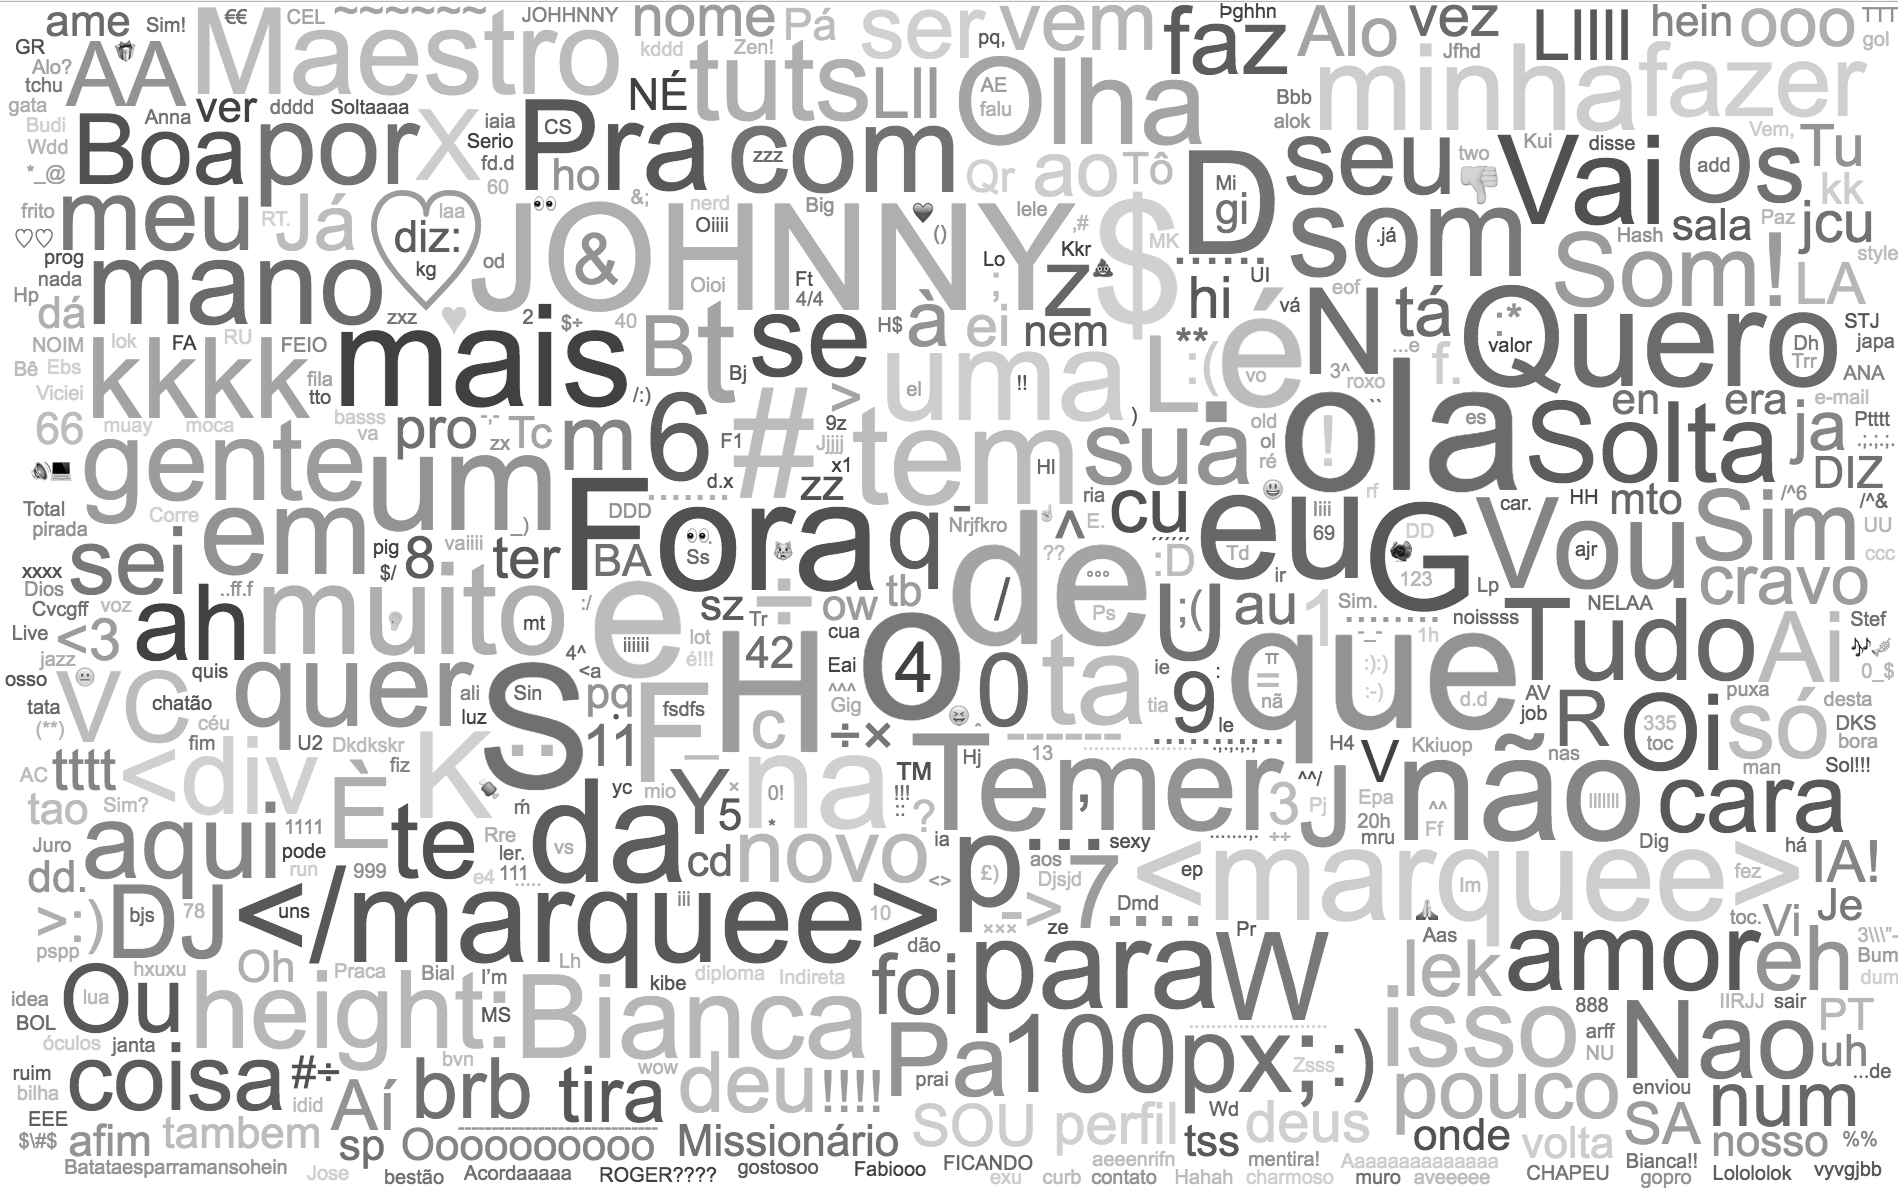
\includegraphics[width=1\linewidth]{pictures/cap3/wordcloud_pb}
\caption{Nuvem de tags gerada pelas palavras utilizadas nas performances analisadas. (Gerada pela autora utilizando a ferramenta Word Cloud).}
\label{fig:cloud}
\end{figure}

A análise revelou que uma grande quantidade de \emph{tokens}, eram palavras de apenas um caractere, que representavam cerca de 19 dos 30 tokens mais usados. Nós acreditamos que isso se deu pela natureza do projeto, uma vez que cada caractere representava um som, então os participantes poderiam usar desta estratégia para gerar um som específico. 

%The analysis revealed that a large number of tokens are single characters which represent 19 out of the 30 most used tokens. We believe that this relates to the specific nature of the Open Band chat application which turns any single character into sounds. This indicates that intent of participants could either focused on semantic meaning or on the resulting sonorities, which we analyzed further in the thematic analysis.

\subsubsection{Análise temática}
\label{sec:thematic}

Para investigar o conteúdo das mensagens, utilizamos uma metodologia de análise temática proposta por Braun e Clarke \cite{Braun2006}. Inicialmente fizemos uma análise da função linguística das mensagens, e posteriormente analisamos fatores mais relacionados ao seu conteúdo semântico.

%We analyzed the message log data using a thematic analysis following the methodology proposed by Braun and Clarke~\cite{Braun2006}. The analysis was conducted at two levels, one looking at the function of the messages, the other looking more closely at the semantic content.

%\subsubsection{Functional analysis}

Inicialmente, identificamos dois grandes grupos de mensagens, um com mensagens com conteúdo semântico explícito, e outro cujas mensagens não pareciam ter conteúdo semântico. As mensagens do primeiro grupo foram divididas nos seguintes grupos:

%We first identified two major groups of messages, depending on whether they included explicit semantic content or if their content was not semantical. The semantic messages were categorized according to their functions, as follows:

\begin{description}
\item[Fática] -- mensagens utilizadas com a principal função de testagem do canal, como:``Oi", ``Olá", etc.
\item[Metelinguística] -- mensagens que referenciavam o projeto ou a performance propriamente dita, como comentários e elogios, por exemplo.
\item[Denominante] -- mensagens que identificavam indivíduos, que podiam ser membros da audiência ou celebridades.
\item[Política] -- mensagens com conteúdo político.
\item[Onomatopaica] -- mensagens com onomatopéias em português ou palavras representando sons.
\item[Risadas] -- mensagens com expressões de risada, um tipo específico de onomatopéia, que foi separado do grupo pela quantidade significante de mensagens. 
\item[Declarações] -- declarações ou afirmações em geral; esta categoria inclui um conteúdo discursivo mais variado.
\item[Código] -- mensagens com códigos de programação ou comandos para mudar os sons.
\item[Emoticons] -- mensagens com emoticons pictóricos, que não eram mapeados em sons, e mensagens formadas por emoticons desenhados por caracteres.
\end{description}

As mensagens de conteúdo não semântico foram divididas em três subgrupos:

\begin{description}
\item[Letras únicas] -- mensagens consistindo de apenas um caractere.
\item[Padrões] -- mensagens que incluíam repetições de caracteres ou de sequências de letras, como um loop de letras.
\item[Aleatórios] -- sequências de caracteres sem lógica.
\end{description}

\begin{figure}[ht!]
\centering
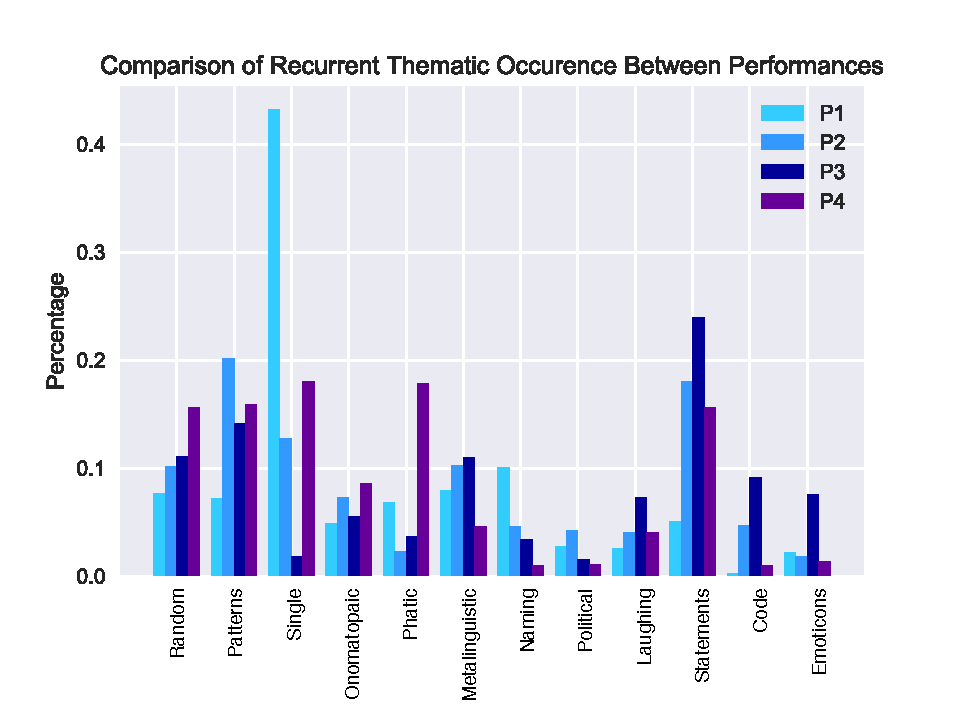
\includegraphics[width=1\linewidth]{pictures/cap3/bar_plot_new_revised}
\caption{Gráfico mostrando as proporções dos temas recorrentes nas performances.}
\label{donut}
\end{figure}

O gráfico representado na Figura \ref{donut} mostra a proporção de mensagens em cada tema identificado na média das performances. De uma maneira geral, podemos notar que a maior quantidade de mensagens em todas performances foram as mensagens de caracteres sozinhos. Nós pudemos também notar que as audiências tiveram comportamentos diferentes com relação à proporção de temas durante as performances. Por exemplo, na performance p1, os caracteres sozinhos foram mais explorados, enquanto na p3 foram menos, mensagens de conteúdo de código foram mais utilizadas na p3, onde a audiência era de cientistas da computação.

\begin{figure}[ht!]
\centering
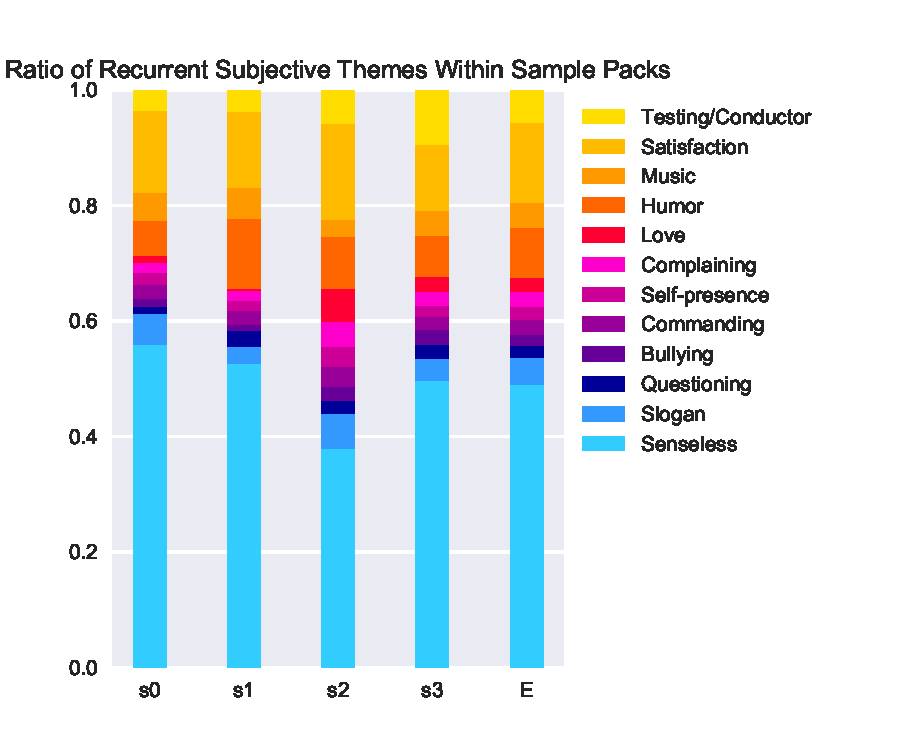
\includegraphics[width=1\linewidth]{pictures/cap3/subj_themes}
\caption{Gráfico mostrando as proporções dos temas subjetivos nas performances.}
\label{donut}
\end{figure}


 %the proportion of the messages in each of the identified themes considering all the performances on average. Overall we can see that messages containing a single character is the most dominating theme. We can note that the audience had different behaviors in respect of the proportion of themes used during the performances. For example, much more exploring "single character'' messages in p1 and less in p3, and much more use of "code'' in p3.  

Depois de categorizar as mensagens em temas de acordo com suas funções linguísticas, fizemos uma nova análise temática, desta vez procurando buscar mais especificamente mensagens de suporte ou crítica, e também com a tentativa de perceber diferenças de comportamentos entre os diferentes conjuntos de samples. Nós identificamos os seguintes temas\footnote{Os temas não são exclsivos, podendo ser aplicados a mais de uma menagem, número total de mensagens entre parêntesis}: sem sentido (1989), slogans (180), questões (73), bullying (77), imperativo (99), auto-presença (81), reclamações (89), amor (84), humor (284), música (174), satisfação (518), e teste/condução (237). Exemplos incluem slogans (e.g. ``Do it"), amor (e.g. ``Paz e amor"), expressões de auto-presença (e.g.``Estou online"), referencias a outros músicos (``Lady gaga") e programas de TV (``Winter is coming" referência à série Game of Thrones), questões (``tem alguém aí?"). 

%After categorizing the messages into functional themes, we further analyzed their content to search for differences in expressions of support from the audience and how the sample packs affected the nature of the messages. We identified  the following (non exclusive) themes (total number of messages reported in brackets): senseless (1989), slogan (180), questioning (73), bullying (77), commanding (99), self-presence (81), complaining (89), love (84), humor (284), music (174), satisfaction (518), and testing/conduction (237). Examples include slogans (e.g. ``Do it"), love (e.g. ``Paz e amor": `` Peace and love"), expressions of self-presence (e.g.``I'm online"), references to musicians (``Lady gaga") and TV shows (``Winter is coming" referring to the Game of Thrones series), questions (``Is there anybody out there?"). %Some out of context copy/pasted text also appeared on the logs now and then.

\begin{table}[ht!]
\tabcolsep8.1pt
\caption{Tabela de frequência de mensagens em cada performance (p) e cada pacote de samples (sp)}{
\begin{tabular}{ c|c|c|c|c|c  }
        & \multicolumn{4}{ c| }{Performance} \\ 
  Pacote de samples & p1 & p2 & p3 & p4& TOTAL\\ \hline     
  sp0   &613 & 430 & 126 & 385 & 1154\\
  sp1   &20 & 81 & 39 & 135 & 275\\
  sp2   &142 & 82 & 143 & 64 & 431\\
  sp3   &783 & 256 & 286 & 139& 1464 \\ \hline
  TOTAL &1558& 849 & 594 & 723& 3724\\
\end{tabular}}
% \begin{tabnote}
% Crosstable of Message Occurrence Per Sample Pack (sp) and Performances (p).
% \end{tabnote}
\label{tbl:perf_sample_xtab}
\end{table}

%\subsection{Link Between Message Content and Sample Pack}

Para investigar como os conjuntos de samples afetaram a natureza e o conteúdo das mensagens enviadas pelos participantes, separamos as mensagens enviadas em cada conjunto de samples (ver Tabela \ref{tbl:perf_sample_xtab}). No total, foram 3724 mensagens enviadas no total pelo sistema. 

%In order to investigate how the various sample packs affect the nature and content of messages sent by participants, we broke down the amount of unique sent messages according to the sample pack (sp) to which they were associated (see Table~\ref{tbl:perf_sample_xtab}). In total, there were 3724 written messages sent during all four performances with various proportions for each sample pack. 


\begin{figure}
\centering
\includegraphics[width=1.1\linewidth]{pictures/cap3/p_val}
\caption{Frequências de conteúdos por pacote de sample.}
\label{subj_themes}
\end{figure}

A Tabela \ref{subj_themes} apresenta a frequência dos temas entre os conjuntos de samples. Usamos análise estatística para checar se haviam diferenças entre a frequência dos temas de acordo com a mudança de conjunto de samples durante as performances. Como a quantidade de mensagens e o tempo de cada conjunto de samples era variável entre as apresentações, comparamos as frequências dos temas utilizando um teste qui-quadrado de independência. Como referência, utilizamos testes estatísticos descritos em \cite{beasley1995multiple} e \cite{garcia2003cellwise}. 

%Table \ref{subj_themes} presents the content theme frequencies across sample packs. Several differences can be noted and their significance was tested using statistical analyses. A Chi-square test of independence was calculated to compare the theme frequencies across sample packs. A significant interaction effect was found ($\chi^2$ (33) = 181.97, $p < .00001$). We performed the post-hoc test described in \cite{beasley1995multiple} and \cite{garcia2003cellwise} using Bonferroni adjusted alpha levels of 0.001.

\begin{figure}
\centering
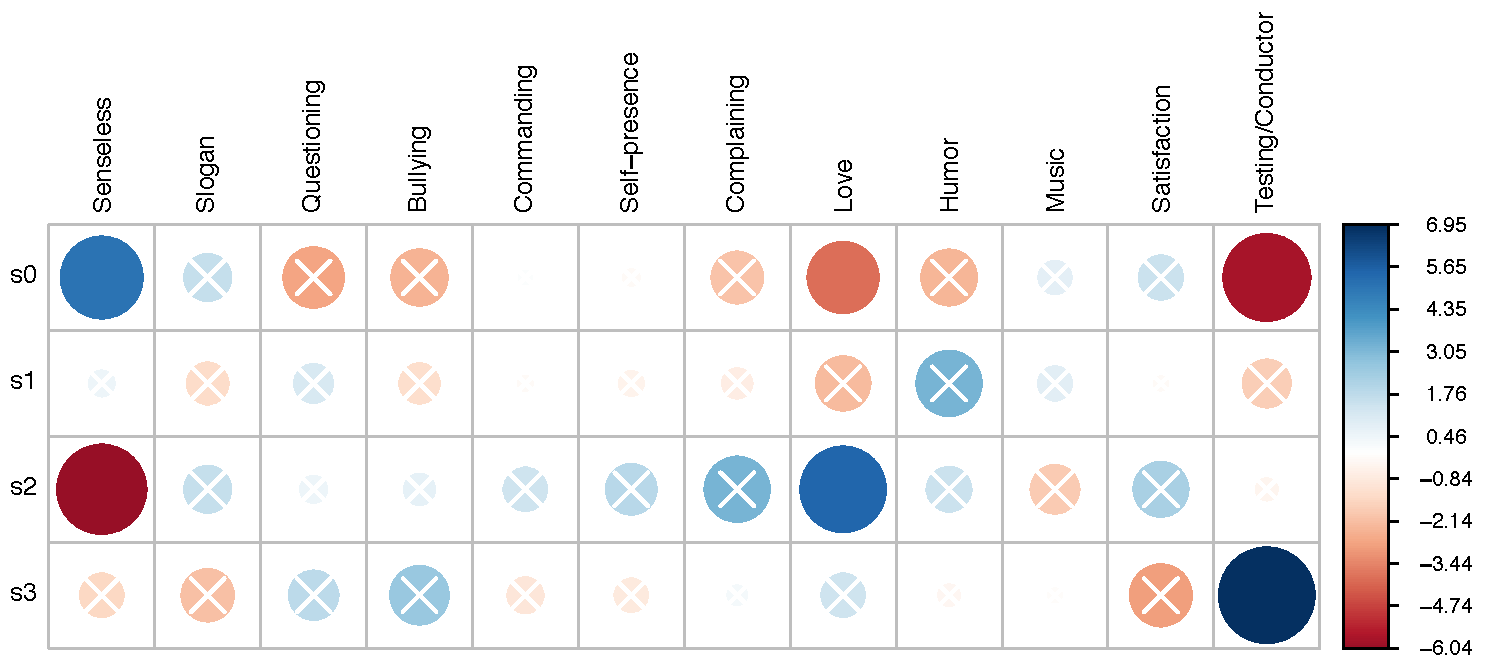
\includegraphics[width=1\linewidth]{pictures/cap3/p_values}
\caption{Variação na frequência de temas entre pacotes de samples. O tamanho dos círculos representa o tamanho do resíduo padrão (quanto maior o círculo, maior a diferença de frequência). A gradação de cor representa diminuição (vermelho) e ampliação (azul).}
\label{fig:bblplot2}
\end{figure}

A Figura \ref{fig:bblplot2} mostra as variações entre frequências de temas entre pacotes de samples, expressa pelo tamanho do resíduo padrão. As diferenças mais significativas foram encontradas entre os conjuntos sp0 e sp2. no caso do conjunto 0 (galáxias), mensagens sem sentido foram mais frequentes do que nos demais samples, e mensagens de amor menos. Isto talvez possa ser explicado pelo fato de que os sons mais estranhos estivessem nos caracteres especiais e numerais, fazendo com que os participantes exploram efeitos sonoros utilizando esses caracteres, que criaram um contraste com os demais sons vocais. Quanto ao sp1 (percussão e acordes), não houve diferença significante, isso pode ser porque ele foi usado menos tempo durante todas as performances, por desejo dos próprios condutores, pois os sons eram mais repetitivos e tradicionais. O conjunto sp2 (colaborativo) apresentou mais mensagens de amor e menos mensagens sem sentido, o que pode ser devido ao fato de não haver uma correlação esperada entre sons e letras. Isso pode ter feito com que os participantes usassem mais discurso formal ao invés de experimentarem com padrões de ritmo. 

De fato, os conjuntos sp0 (Galáxias), sp1 (Percussão e Acordes) e sp3 (Orquestra Errante) foram produzidos por um método mais rigoroso de tradução intersemiótica, e foram os que levaram a mais experimentação fora do campo do discurso nas performances analisadas. 

%Figure~\ref{fig:bblplot2} displays the sources of variations of theme frequency across sample packs expressed as the size of the standardized residual. The post hoc analysis showed that significant differences of theme frequency occurred for Sample Packs 0 and 2, and for Sample Pack 3, to a lesser extent. With sp0 differences were obtained for the themes 'Love', 'Senseless' and 'Testing/Conductor' ($p < .001$). As Figure ~\ref{fig:bblplot2} shows, 'Love'-themed messages were less frequent for sp0 while 'Senseless'-themed messages occurred more frequently. This may be explained by the fact that for this sample pack, special characters were  mapped to sound effects creating unexpected contrasts compared to letters that were associated to vocal sounds. Participants may have preferred to use the special characters for these reasons leading to a more frequent occurrence of messages without semantic meaning (senseless).

%No significant changes were found for sp1. This may be because this sample pack was on overall less used for musical purposes, given that its sounds are repetitive and conductors preferred to use the pack for introduction to the system and short durations. Contrary to sp0, for sp2 'Love'-themed messages were used more frequently and there were less 'Senseless' messages in this sample pack. This may come from the fact that for this sound pack there is no expected association between letters and sounds. Participants may hence have employed a more discursive style instead of exploring letter to sound association in a rhythmic way like for other sample packs. Indeed the sample packs sp0, sp1 and sp3 which were composed using a rigorous inter-semiotic translation approach (see Section ) lead more consistently to non-semantic expressions in the chat system, contrasting with sp2 which includes sounds composed collaboratively. For sp3, the only significant difference was related to the 'Testing/Conductor' theme. As sp3 was used mostly at the end of the pieces, this is connected to the commands entered by conductors to direct the closure of the performances.

Não houve nenhuma variação significativa na frequência dos temas ``satisfação'', ``humor'' e ``reclamações'' entre os pacotes de samples, o que pode demonstrar que o grau de satisfação não foi significativamente alterado ou pelo menos não foi registrado pelos participantes de uma maneira geral. 

%There weren't any significant theme frequency variations for 'Satisfaction', 'Humor' and 'Complaint' messages between sample packs. This may indicate that the choice of sample packs did not influence the overall hedonic experience of the participants.



%\subsection{Design}

%Various text-to-sound mappings were investigated throughout the development of Open Band: by (i) mapping letters to sounds using sample-based synthesis ~\cite{Stolfi2017} following a procedure of inter-semiotic translation~\cite{JulioPlaza1969}, or by (ii) using web audio synthesis following an isomorphic relation between the sound spectrum and the letters~\cite{Stolfi2017b}. In both cases, the mappings between the letters and the sounds were established a priori by the author and experimenters, so the only creative sonic control for the audience consisted in proposing combinations of sounds over time. Although analyses of data collected during performances indicated that the experience was fun and engaging for the audience~\cite{Stolfi2018}, we found that the capabilities of the system to support creative musical composition were limited due to the constraints and limited sonic agency. 


\subsubsection{Conclusões}


Um dos nossos objetivos era de prover uma plataforma para livre expressão da audiência, como uma ``web ágora''. Como atestar isso de uma maneira científica foi uma questão que norteou o processo de análise que envolveu processos quantitativos (de análise estatística) e qualitativos (análise temática). A diversidade de temas que surgiram nas análises indicam que este objetivo foi atingido, uma vez que os participantes expressaram diversas posições e discutiram temas que variaram de amor a opiniões políticas divergentes, expondo também preconceitos e \emph{nonsense}.

A análise temática das mensagens, revelou um grande grau de suporte dos usuários, que pudemos medir pela quantidade significante de mensagens e satisfação (cerca de 14\% de todas mensagens). A quantidade de mensagens também indica um grande engajamento do público, com mais de mil mensagens enviadas a cada performance (ver tabela \ref{tab:msgtype}). Esses dados indicam que a plataforma foi acessada com facilidade e acessibilidade, mesmo em casos onde a audiência não tinha necessariamente conhecimentos musicais prévios. 

%One of our design goals was to provide a platform for free audience expression as a web ``agora". The various themes which emerged from the analyses endorse this idea as participants felt free to discuss subjects ranging from love to political opinions.

%The thematic analysis revealed a high degree of appreciation and support from participants; the second most frequently occurring theme was 'Satisfaction' with 518 messages across performances (14\% of all messages). Log data analyses revealed that participants actively engaged in the performances as over a thousand messages were played in each performance (see Table \ref{tab:msgtype}). Such behavior and the expressions of support in the chat communication are signs that the tool was easily accessible by audience members and that no previous musical knowledge is necessary to engage with it.

Ficou claro que a interface de chat encorajou os participantes a usar a plataforma como um meio de comunicação para conversarem entre si, mas apesar das semelhanças que o sistema pode ter com outros sistemas de comunicação online, quase metade das mensagens escritas não tinham significado semântico. Essas mensagens, que dividimos em três subcategorias (caracteres sozinhos, padrões e aleatórias) indicam que a audiência também utilizou o sistema para explorar o sistema de forma musical, explorando ritmos e sons de maneira estética.

%The two categories of semantic and non-semantic messages appear in almost equal proportions across performances. It is clear that the chat interface encouraged participants to use Open Band as a way to communicate with each other. Screen projection of the chat made Open Band a compelling means for posting messages to be shared with ones's entourage, as is done in other social media platforms. However, although Open Band's interface shares similarity with other web-based platforms for verbal communication, approximately half of the messages did not show any explicit semantic content. These messages, which can be divided into three sub-categories (single characters, patterns, and random-like) point to the exploration of the musical potential of Open Band, since they served to engage with the system's sonic features and to performatively explore these features.

Tocar repetidamente a mesma letra pode ser visto como uma forma de testar o sistema, mas também como forma de disparar sons em um ritmo específico, e também de ouvir aquele som único no meio da massa sonora composta pelas frases. é similar à função fática no contexto semântico, como aponta Jakobson que serve principalmente para estabelecer, prolongar ou encerrar a comunicação \cite{Jakobson}. Também permite com que os usuários reconheçam a sua contribuição específica dentro da performance e reconhecer os sons individuais. Padrões, por outro lado, ou repetições de sequências curtas permitem aos participantes a criação de motivos rítmicos ou frases musicais, que também se destacam do conteúdo textual que em geral não tem muita repetição, se aproximando da linguagem musical.

%Repeatedly typing the same letter can be seen as a way to test the system and check its communicative capabilities. It is similar to the phatic function in the semantic context ``primarily serving to establish, to prolong, or to discontinue communication" \cite{Jakobson}. By repeating a same keyboard key the user could recognize the relationship between individual letters and the sounds they produce. In addition, repetition allows a clear identification of each participant's own sonic contribution within the somewhat complex flow of sounds that can be produced during a performance. On the other hand, the loop repetition of short sequences allows for the creation of rhythmic motifs that stand out from the random sonorities produced at certain moments. Finally, texts with non-semantic content produced by the almost random triggering of the keys are strong indicators of participation in performing Open Band as a music practice.

Como aponta uma das mais importantes referências da cultura moderna brasileira nas artes, o Manifesto Antropofágo de Oswald de Andrade de 1928 \cite{Andrade1928}, ``a alegria é a prova dos nove''. Nesse sentido, os dados recolhidos, assim como a observação do comportamento da audiência apontam uma evidência de que o projeto foi bem sucedido nesse sentido, com várias referências de humor, declarações de apoio e risadas registradas pela audiência. 

%Possibly one of the biggest influences in Brazilian modern culture, the 1928 ``Cannibal Manifest" from poet Oswald de Andrade~\cite{Andrade1928} presents an important standpoint for our work, ``Joy is the real proof". From this standpoint the data provide some evidence that the performances were experienced in a playful way, as there were many statements and declarations of fun and enjoyment in participant messages.

Sob outro ponto de vista, que era o de propor uma ``Obra Aberta'', nós consideramos que o sistema poderia ser mais aberto, uma vez que os usuários tinham liberdade somente para escolher o texto, mas não para fugir dos sons pré-programados pela compositora e escolhidos pelo condutor durante as performances. Em se tratando de uma audiência que não tinha necessariamente treinamento musical, essa opção foi importante para manter a consistência estética do projeto.

%From another standpoint, which was to propose an Open Work, we still consider the current system insufficient, as users have little freedom about the sounds to use since these are restricted to the ones chosen by the composer and the conductors during the performance. We maintained the control of sound production mechanisms fairly simple in favor of ease of use and intuitiveness. With such an approach the system is open to audience without prior musical knowledge, thus minimizing the amount of instructions required to participate. To maintain artistic consistency of live performances, the sample packs' choices were left to the artists facilitating the performances. %The choice of constraints was also decided to maintain the artistic consistency of the live performances in musical terms.



%However to increase the agency of participants, users should be able to map themselves the sound into letters, or at least be able to decide between broader sound options. To attempt to address this issue, we are developing as part of the Audio Commons\footnote{\url{http://audiocommons.org}} project, a new platform using the Freesound Application Programming Interface~\cite{Font2013}. The prototype, Playsound.space, is a web-based interface (Figure ~\ref{playsound}) that let users search sounds in the Freesound database using semantic queries. Future work will investigate how letters can be mapped into sounds in the Playsound platform. Combining the Open Band and Playsound frameworks may lead to new interesting applications for the re-purposing of crowd-sourced content for music making and instant messaging auditory display.


%We wanted to expand it to be a framework to be used in different musical contexts. One of our goals is to integrate the project with the audio Commons API\cite{Akkermans2011} to foster media re-purposing, creating an interface for uploading and mapping sounds to the letters. For the web audio synthesis version, we aim to develop form to control the base frequencies and rhythm trough gestural interfaces, to enhance the musical possibilities given to the audience.

Apesar do projeto Banda Aberta ter se mostrado interessante como experiência participativa e projeto de performances, os resultados sonoros e as possibilidades criativas de produção musical ainda não estavam suficientes para suprir necessidades pessoais individuais. Como performance participativa, foi interessante porque demonstrou que o texto podia ser uma forma fácil e intuitiva de interação musical. Considero que a experiência do projeto Banda Aberta foi interessante como possibilidade de explorar uma composição musical interativa, e também de explorar um processo compositivo de montagem sonora coletiva, mas com um nível de constrição muito alto. 

A experiência foi bastante importante também para demonstrar as capacidades de processamento, controle e acessibilidade das tecnologias web para práticas musicais. Em nenhuma das apresentações realizadas, sob diversas condições de aparelhagem e sistemas de som, consideramos que a qualidade sonora fosse suficiente. O sistema também se mostrou muito versátil e adaptável à mobilidade e condições diversas de aparelhagem de som. Em um caso extremo, no festival  Áudio Insurgência, a mesa de som da casa estava com defeito, e tivemos que ligar o sistema direto do celular com um cabo p10/RCA.

Como um instrumento para performance ao vivo, no entanto, ainda me parecia insuficiente. Durante minhas atividades práticas musicais, tive a oportunidade de tocar com o sistema em performances de improvisação livre em algumas situações, como na apresentação para o festival aMostra Sonora. Durante a performance, onde utilizei também um patch de Pure Data que desenvolvo há cerca de 10 anos, percebi que a quantidade de sons não era suficiente para proporcionar uma variação sonora satisfatória em performances longas. O sistema, que é propositalmente simples, para que seja o mais leve possível, não permite processamentos mais complexos do som, e por mais que o conjunto de sons fosse grande, a falta de controle em fatores mais sutis, que são importantes em uma performance solo de improvisação musical me deixaram entediada com o sistema durante a apresentação. Para isso, precisaria também de algo que realmente servisse como um instrumento musical, e não somente como um mapeamento fixo. 

A partir daí, surgiu a idéia de um projeto que envolvesse a API do Freesound, que inicialmente pensava como um framework que expandisse as potencialidades sonoras deste projeto. A idéia inicial foi o de usar a API do Freesound como um método para mapear os sons em letras, que iriam ser acessadas dentro do sistema do Banda Aberta. Para conseguir desenvolver essa tecnologia, escrevi um projeto para um estágio de pesquisa junto ao Centre for Digital Music (C4DM) da Queen Mary University of London (QMUL),  sob orientação do professor Mathieu Barthet, uma vez que lá havia um dos grupos de trabalho do projeto Audio Commons, que entre outras coisas, estava dando suporte ao Freesound. 


%- amostra - limitação de sons para performances longas
%- audio mostly - feedback atrapalhou a performance


\end{otherlanguage*}



